\documentclass[pdfpaper,openbib, twoside, titlepage, halfparskip-,a4paper, 10pt]{scrarticle}
\usepackage{siunitx}
%\usepackage[a4paper,left=2cm,right=2cm,top=3cm,bottom=3cm]{geometry}
\usepackage[left=2.5cm, right=2.5cm, top=2.5cm, bottom=2cm, footnotesep=1cm,includeheadfoot]{geometry}
\usepackage[ngerman]{babel}
\usepackage{amsthm}
\usepackage{amssymb}
\usepackage{pdflscape}
\usepackage{amsmath}
\usepackage{needspace}
\usepackage{amsfonts}
\usepackage{biblatex}
\usepackage{array}
\usepackage{graphicx}
\usepackage{tabularx}
\usepackage{pdfpages}
\usepackage{colortbl}
\usepackage{hyperref}
\usepackage{booktabs}
\usepackage{tikz}
\usepackage{xcolor}
\usepackage{lscape}
\usepackage{multirow}
\usepackage{float}
\usepackage{caption}
\usepackage{rotating}
\usepackage{listings}
\definecolor{lightgreen}{RGB}{198, 239, 206}
\definecolor{lightgray}{gray}{0.95}
\usetikzlibrary{shapes.geometric, arrows.meta, positioning, calc}
\tikzstyle{process} = [rectangle, draw, minimum height=2.5em, minimum width=3.5em, align=center]
\tikzstyle{arrow} = [->, >=latex]
\tikzstyle{label} = [align=left]
\hypersetup{
    colorlinks=true,
    linkcolor=blue,
    filecolor=blue,      
    urlcolor=blue,
    citecolor=blue,
    pdftitle={Bericht_Due_Hoh_Kon_Ste_Wal},
    }
\addbibresource{Literaturverzeichnis.bib}


\title{VTP Gebläse Venturi}
\author{Marc Hoheisel}
\date{\today}

\usepackage[headsepline,footsepline]{scrlayer-scrpage}
\pagestyle{scrheadings}
\ihead{VTP Gebläse Venturi}
\ohead{
\includegraphics[scale=0.05]{Bilder/HM_Logo_RGB.png}}
\chead{}
\ifoot{\headmark}
\cfoot{}
\ofoot{\pagemark}
\automark[subsection]{section}  % \automark[rechte Seite]{linke Seite}
\begin{document}

% für Abbildung von Matlab code
\lstset{
  language=Matlab,
  basicstyle=\ttfamily\small,
  commentstyle=\color{gray},
  mathescape=true,              % Aktiviert $...$ in Kommentaren
  keywordstyle=\color{blue},
  stringstyle=\color{red},
  numbers=left,
  numberstyle=\tiny\color{gray},
  breaklines=true,
  frame=single
}

\begin{titlepage}
\begin{figure}
\begin{flushleft}
    
    
\includegraphics[width=0.3\linewidth]{Bilder/HM_Logo_RGB.png}
\end{flushleft}
\end{figure}
\text{Prof. Dr.-Ing Bernhard Simon} \\
\text{Fakultät für Maschinenbau, Fahrzeugtechnik, Flugzeugtechnik}
\mbox{}\\
\vspace{2cm}
\begin{center}
\begin{flushleft}
\Huge
    \textbf{Versuchstechnisches Praktikum Gebläse und Venturi}\\
\normalsize
\vspace{1cm}
\text{Praktikumsbericht \today} \\
<<<<<<< HEAD
%\text{Versuchsgruppe: XY}
=======
>>>>>>> f7e2758e2eda898a4889a4c273cdbaf1a29be930
\end{flushleft}
\end{center}

%\begin{figure}
%\center
%\textbf{\Large Bestätigung der eigenständigen Berichterstellung durch Teilnehmer}
%\begin{center}
%\begin{tabular}{|
%>{\centering\arraybackslash}m{3.8cm}|
%>{\centering\arraybackslash}m{4cm}|
%>{\centering\arraybackslash}m{3cm}|
%>{\centering\arraybackslash}m{3.5cm}|
%>{\centering\arraybackslash}m{3.5cm}|}
%\hline

%\textbf{Name} & \textbf{Unterschrift} & \textbf{Matrikelnummer} & \textbf{Studiensemester}\\
%\hline
%Marc Hoheisel & \includegraphics[width=3cm]{UnterschriftHoheisel.pdf} & 29706923 & LRB 4 \\
%\hline 
%Elias Dürrwanger & \includegraphics[width=3cm]{Unterschrifteduerrwanger.pdf} & 04342923 & LRB 4 \\
%\hline 
%Kirill Konorov & \includegraphics[width=3cm]{Unterschriftkonorov.pdf} & 36432423 &LRB 4  \\
%\hline 
%Thomas Walter & \includegraphics[width=3cm]{Unterschriftwalter.pdf} & 50329323 & LRB 4 \\
%hline 
%Laurin Steinebach & \includegraphics[width=3cm]{Unterschriftsteinebach.pdf} & 63601721 & LRB 4 \\
%\hline
%\end{tabular}
%\end{center}
%\end{figure}


\vspace{3cm}
\begin{flushleft}
\textbf{Filipp Brummet} \\
\vspace{0.25cm}
\textbf{Roberto Sessa} \\
\vspace{0.25cm}
\textbf{Marc Hoheisel} \\
%Email: m.hoheisel@hm.edu\\
%Matr.-Nr.: 29706923\\
\end{flushleft}
\end{titlepage}
\tableofcontents
\newpage

\section{Gebläse}
\subsection{Einleitung / Abstract}
Ziel des vorliegenden Versuchs ist die experimentelle Untersuchung des Betriebsverhaltens eines doppelflutigen Radialgebläses. Hierzu werden sechs unterschiedliche Drosselstellungen mit Austrittsdurchmessern im Bereich von 0 mm bis 200 mm betrachtet. Für jede Drosselkonfiguration erfolgt eine Variation der Drehzahl zwischen 1000~min$^{-1}$ und 2800~min$^{-1}$. 

Im Rahmen der Messungen werden das an der Welle anliegende Drehmoment sowie der statische und dynamische Druck erfasst. Auf Grundlage der daraus bestimmten Kennwerte wird eine systematische Analyse und Bewertung der Gebläsecharakteristik unter realitätsnahen Betriebsbedingungen durchgeführt.


\subsection{Versuchsbeschreibung und -durchführung}
\subsubsection{Zielsetzung}
Ziel des Versuchs ist die systematische Analyse des Förderverhaltens sowie der Effizienz eines doppelflutigen Radialgebläses unter praxisnahen Bedingungen. Durch die gezielte Variation der Drehzahl und der Drosselstellung werden charakteristische Kennwerte wie Volumenstrom, Druckanstieg und Wirkungsgrad experimentell ermittelt und anschließend ausgewertet.

\subsubsection{Versuchsaufbau und Beschreibung aller relevanten Komponenten}
Hauptbestandteil des Prüfstands ist ein doppelflutiges Radialgebläse mit spiralig ausgeführtem Gehäuse, das über eine direkt gekoppelte Welle von einem Drehstrommotor angetrieben wird. Die Drehzahl des Antriebs lässt sich mithilfe eines Frequenzumrichters stufenlos einstellen, wobei die Vorgabe manuell über ein Potentiometer erfolgt. Dadurch kann ein breiter Bereich unterschiedlicher Betriebspunkte abgebildet werden.

Zwischen Motor und Laufrad ist eine transparente DMS-Messwelle integriert, mit der das anliegende Drehmoment $M_W$ kontinuierlich erfasst wird. In Kombination mit der gemessenen Drehzahl ermöglicht dies die Bestimmung der mechanischen Wellenleistung $P_W$, welche als Grundlage zur Berechnung des strömungsmechanischen Wirkungsgrads dient.

\begin{figure}[h]
    \centering
    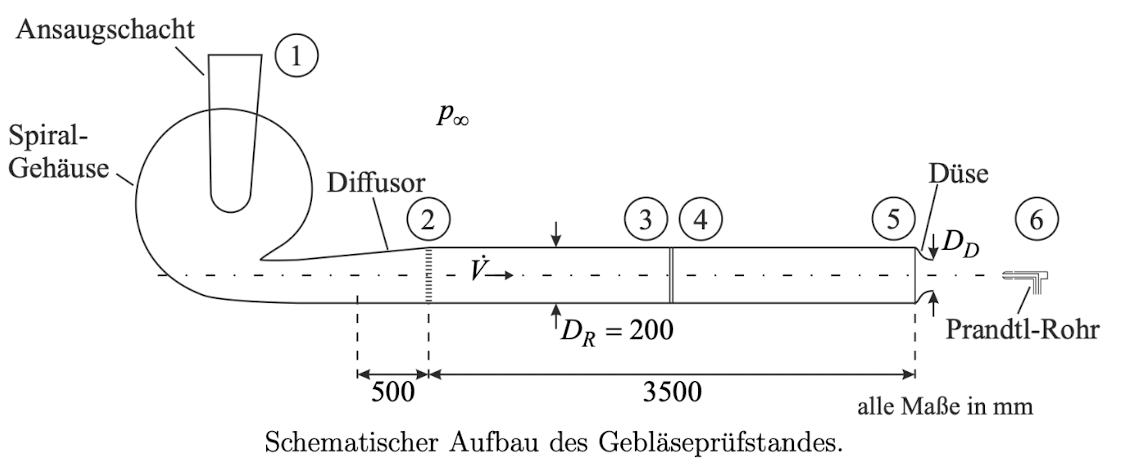
\includegraphics[width=0.9\textwidth]{Bilder/Versuchsaufbau.png}
    \caption{Versuchsaufbau Gebläse}
    \label{fig:versuchsaufbau_gebläse}
\end{figure}

\newpage
\subsubsection{Versuchsdurchführung} 


Wie in Abbildung~\ref{fig:versuchsaufbau_gebläse}dargestellt, saugt das Gebläse die Umgebungsluft zunächst über einen rechteckigen Ansaugschacht (Position~1) an und fördert diese in das angeschlossene Prüfrohr mit einem Innendurchmesser von 200~mm und einer Länge von 3500~mm. \\
\\
Unmittelbar hinter dem Gebläseausgang ist ein Diffusor angeordnet, der durch Reduktion der Strömungs- geschwindigkeit eine Erhöhung des statischen Drucks bewirkt. Der nachgeschaltete Strömungsgleichrichter (Position~2) dient dazu, den am Diffusorausgang vorhandenen Drall zu reduzieren und eine möglichst homogene Strömung im Rohr sicherzustellen. Am Ende des Prüfrohrs können austauschbare Normdüsen installiert werden, mit deren Hilfe der Strömungsquerschnitt gezielt variiert wird. Auf diese Weise lassen sich unterschiedliche Betriebspunkte des Gebläses durch definierte Drosselzustände einstellen. Es stehen Normdüsen mit Austrittsdurchmessern von 200, 100, 80, 50 und 0~mm zur Verfügung, wobei ein Durchmesser von 0~mm einer vollständigen Schließung und 200~mm einer vollständigen Öffnung des Prüfrohrs entspricht. \\
\\
Die Erfassung des statischen Drucks erfolgt über vier gleichmäßig über den Rohrumfang verteilte Druckbohrungen (Position~5), die über eine Ringleitung mit einem elektronischen Drucksensor verbunden sind. Zur Bestimmung des dynamischen Drucks am Düsenaustritt wird ein Prandtl-Rohr (Position~6) eingesetzt, welches ein punktförmiges Messverfahren darstellt.

\subsection{Versuchsergebnisse}
Zuerst wird die Dichte der Luft ermittelt. Dabei wird der Luftdruck, die Luftfeuchtigkeit sowie die Temperatur im Versuchsraum gemessen:
\begin{table}[H]
    \centering
\begin{tabular}{c|c}
    Luftdruck & 955,5 hPa\\
    Luftfeuchtigkeit & 38 \% \\
    Temperatur & 19,6 °C
\end{tabular}
\end{table}
Es wurde eine Luftfeuchtigkeit gemessen von $\varphi = 38 \ \%$. Da diese unter $50 \%$ liegt, wird mit einer Gaskonstante von $R_S = 287,05 \ \frac{J}{kgK}$ gerechnet. 
Mit diesen Werten kann auf die Dichte der Luft geschlossen werden:
\begin{equation}
    \varrho = \frac{p_\infty}{R_S T}
\end{equation}

\begin{equation*}
    \varrho = \frac{95545 \ Pa}{287,05 \ \frac{J}{kgK} \cdot 292,75 \ K} = 1,137 \;\frac{kg}{m^3}
\end{equation*}

Fortlaufend werden sechs, für das Gebläse charakterisierende, Kennlinien ermittelt:
\begin{itemize}
    \item $\dot{V} = \dot{V} (N)$
    \item $\Delta p_{t,12} = \Delta p_{t,12} (N)$
    \item $P_W =P_W(N)$
    \item $\eta = \eta(N)$
    \item $\Delta p_{t,12} = \Delta p_{t,12} (\dot{V})$
    \item $\Psi = \Psi (\varphi)$
\end{itemize}
Die Gleichung zur berechnung des Volumenstrom bei einem offen Rohr $D_D=200\ mm$ und einer Drehzahl von $n=2500 \ \frac{1}{min}$:
\begin{equation}
    \dot{V}= k_1 \cdot c_{6,ax} \cdot \frac{\pi D_D^2}{4} 
\end{equation}
Für die Berechnung des Volumenstroms wird, der dynamische Druck am Düsenende gemessen. Mit diesem Druck kann auf die Geschwindigkeit der Luft geschlossen werden:
\begin{equation}
    c_{6,ax}=\sqrt{\frac{2}{\varrho} \cdot p_6}
\end{equation}
Bei einem dynamischen Druck von $p_6 = 143 \ Pa$ ergibt sich:
\begin{equation*}
    c_{6,ax} = \sqrt{\frac{2}{1,137\frac{kg}{m^3}} \cdot 143 \ Pa} \ = 15,86 \ \frac{m}{s}
\end{equation*}
Weiter wird mit einem Korrekturfaktor von $k_1 = 0,8733$ und der Geschwindigkeit $c_{6,ax}$ der Volumenstrom ermittelt:
\begin{equation*}
    \dot{V} = 0,8733  \cdot 15,86 \frac{m}{s} \cdot \frac{\pi \cdot (0,2 \ m)^2}{4} = 0,435 \ \frac{m^3}{s}
\end{equation*}
Der Korrekturfaktor ist vonnöten, da der dynamische Druck an Punkt 6 nur punktuell gemessen wird und dem entsprechend nicht der Durchschnittsgeschwindigkeit entspricht. Der Korrekturfaktor wurde im Skript \cite{VTP_Beschreibung} vorgegeben.\\
Mit den verschiedenen Düsenöffnungen und Drehzahlen ergeben sich folgende Kennlinien:
\begin{figure}[H]
    \centering
    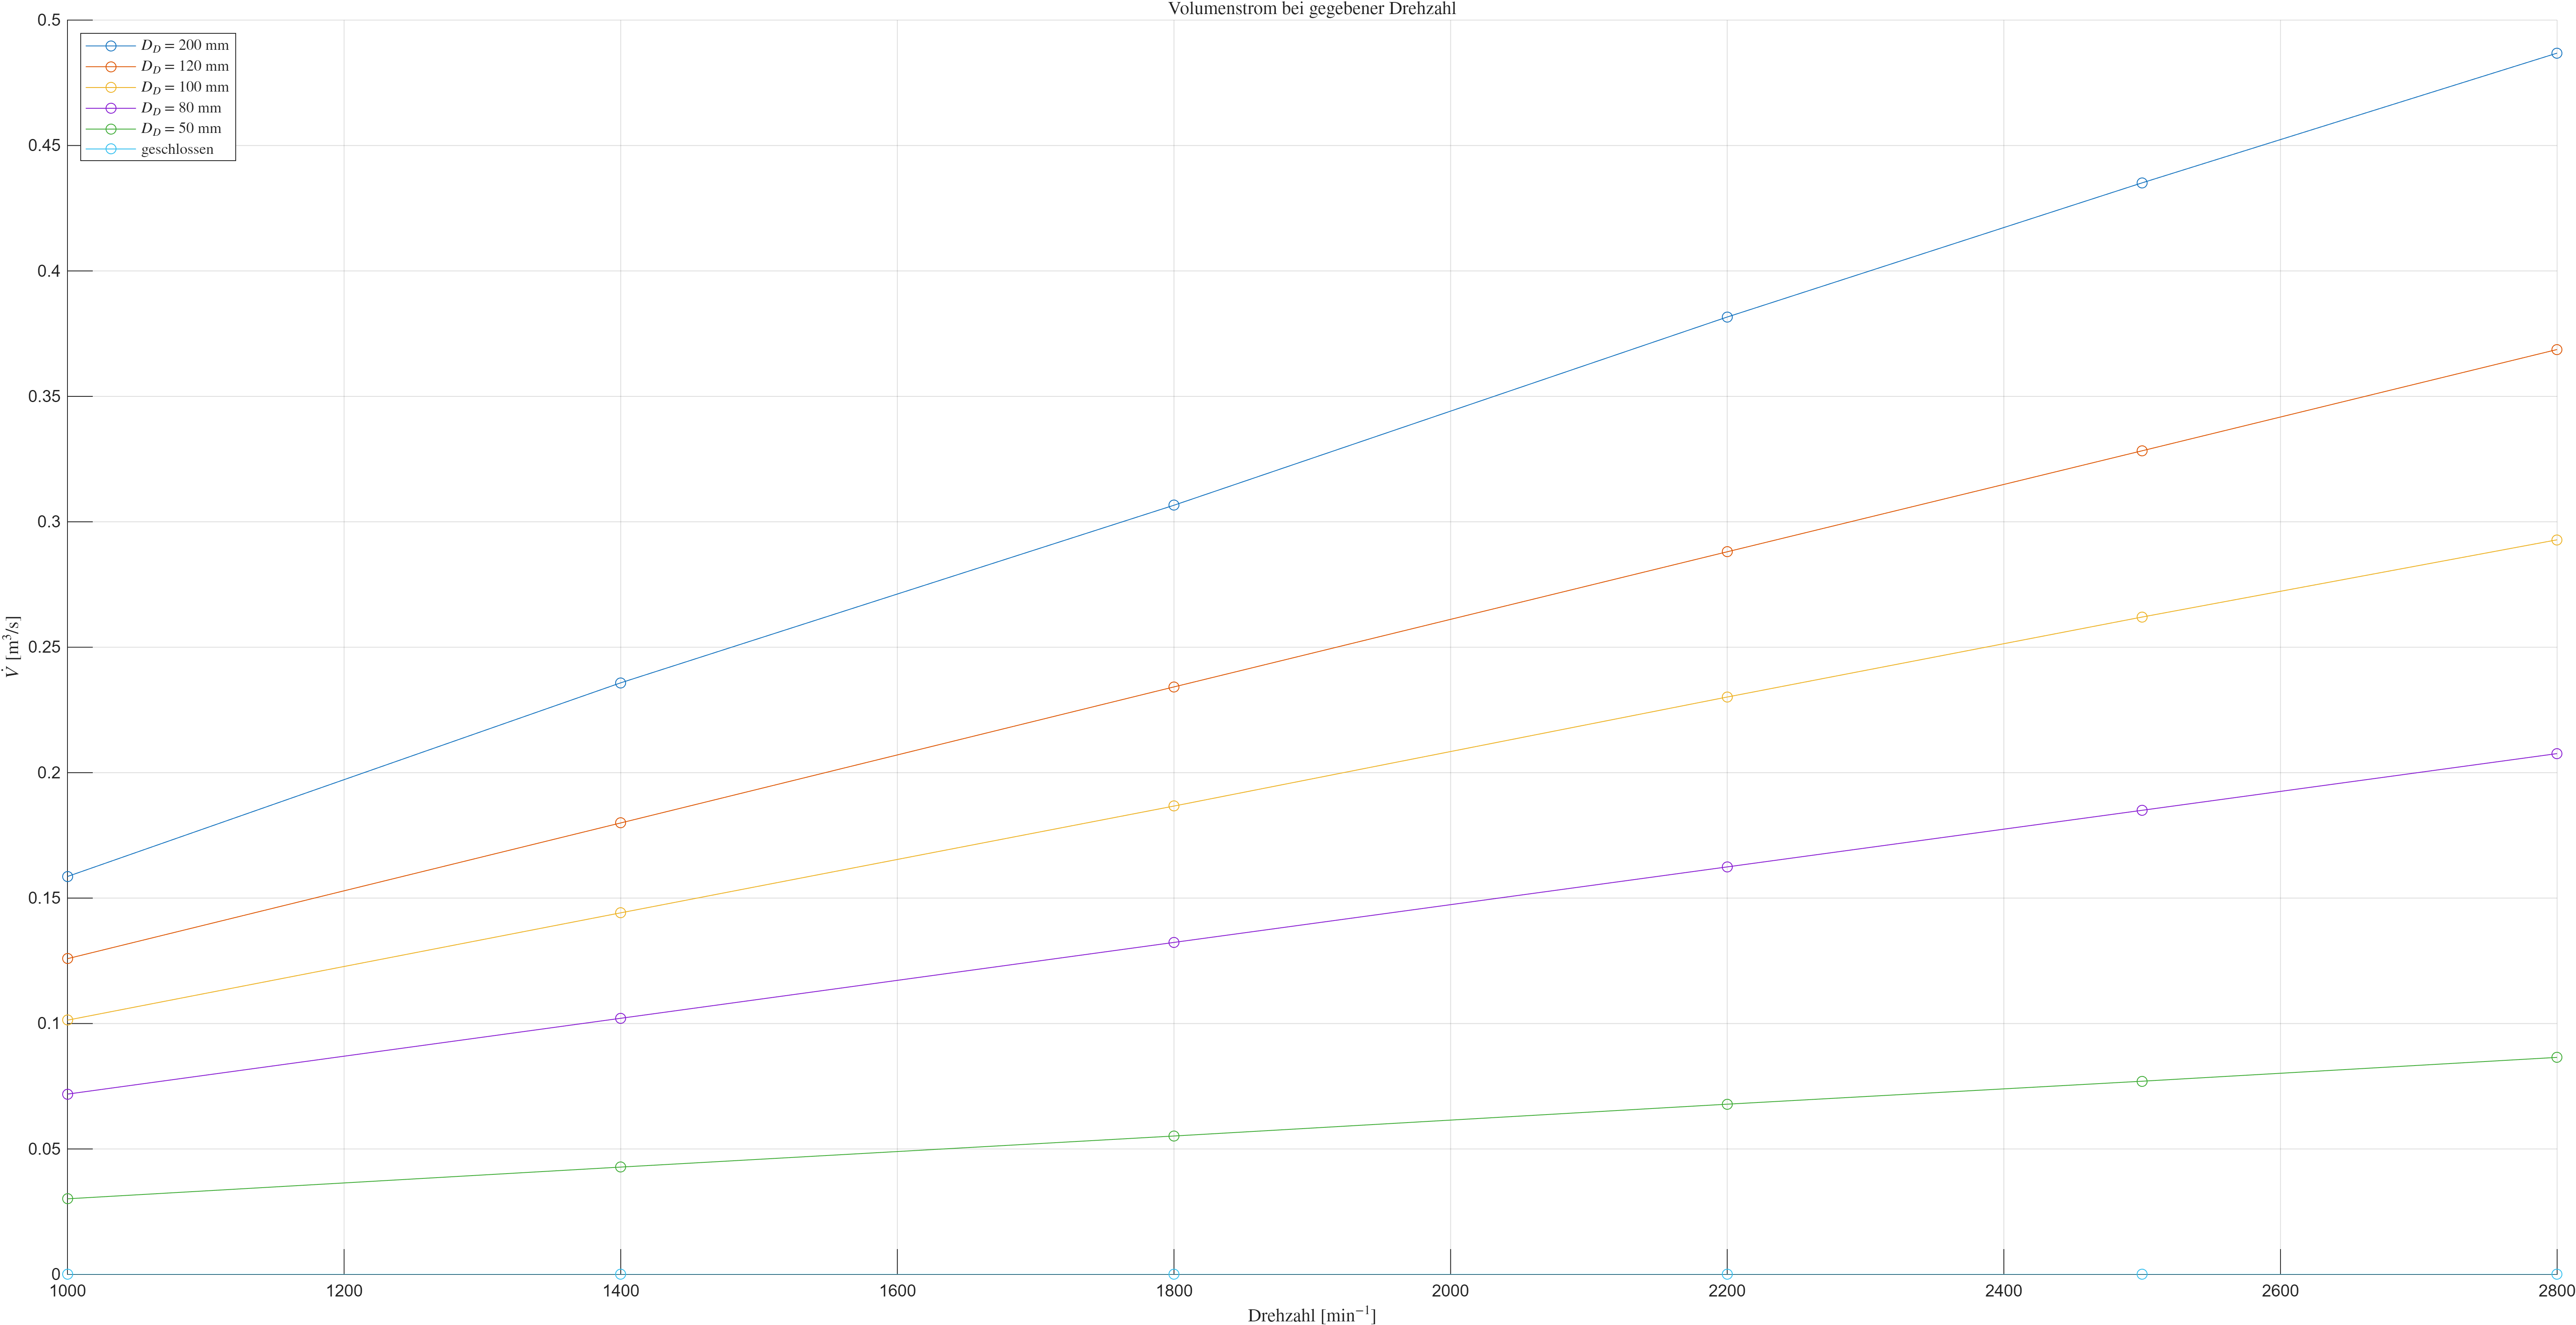
\includegraphics[width = 1 \linewidth]{Plots/Gebläse/Volumentstrom_Plot.png}
    \caption{Volumenstrom in Abhängigkeit der Drehzahl}
    \label{plot:Volumenstrom}
\end{figure}

Berechnung der Totaldruckerhöhung durch das Gebläse:
\begin{align}
    \Delta p_{t,12}&= \frac{\varrho}{2}c_2^2 + p_2 = p_5 + \frac{\varrho}{2}c_5^2 + \zeta \cdot \frac{\varrho}{2}c_5^2, \quad \text{wobei: } \zeta = 0,25 \\
    \Delta p_{t,12}&=p_5 + 1,25 \cdot \frac{\varrho}{2} c_5^2
\end{align}
Diese Gleichung ergibt sich aus der Bernoulli Gleichung wobei bei einem konstanten Rohrquerschnitt gilt: $c_2 = c_5$ und mit berücksichtigung der Druckverluste ergibt sich der Zusammenhang:
\begin{equation}
    p_2 = p_5 + \zeta \cdot \frac{\varrho}{2}c_5^2
\end{equation}
\begin{equation*}
    \Delta p_{t,12}=40 \ Pa + 1,25 \cdot \frac{1,137 \ \frac{kg}{m^3}}{2} \cdot (13,85 \ \frac{m}{s})^2 = 176,3 \ Pa
\end{equation*}

mit $c_5$ der mittleren Strömungsgeschwindigkeit im Rohr, welche mittels der Kontinuitätsgleichung berechnet wird:
\begin{equation}
    c_5 = \frac{\dot V}{A} = \frac{\dot V}{\frac{\pi \cdot D_R^2}{4}}
\end{equation}

\begin{equation*}
    c_5 =  \frac{0,435 \ \frac{m^3}{s}}{\frac{\pi \cdot(0,2 \ m)^2}{4}} = 13,85 \ \frac{m}{s}
\end{equation*}

Bei anderen Drehzahlen und Düsenöffnungen ergeben sich folgende Kennlinien:
\begin{figure}[H]
    \centering
    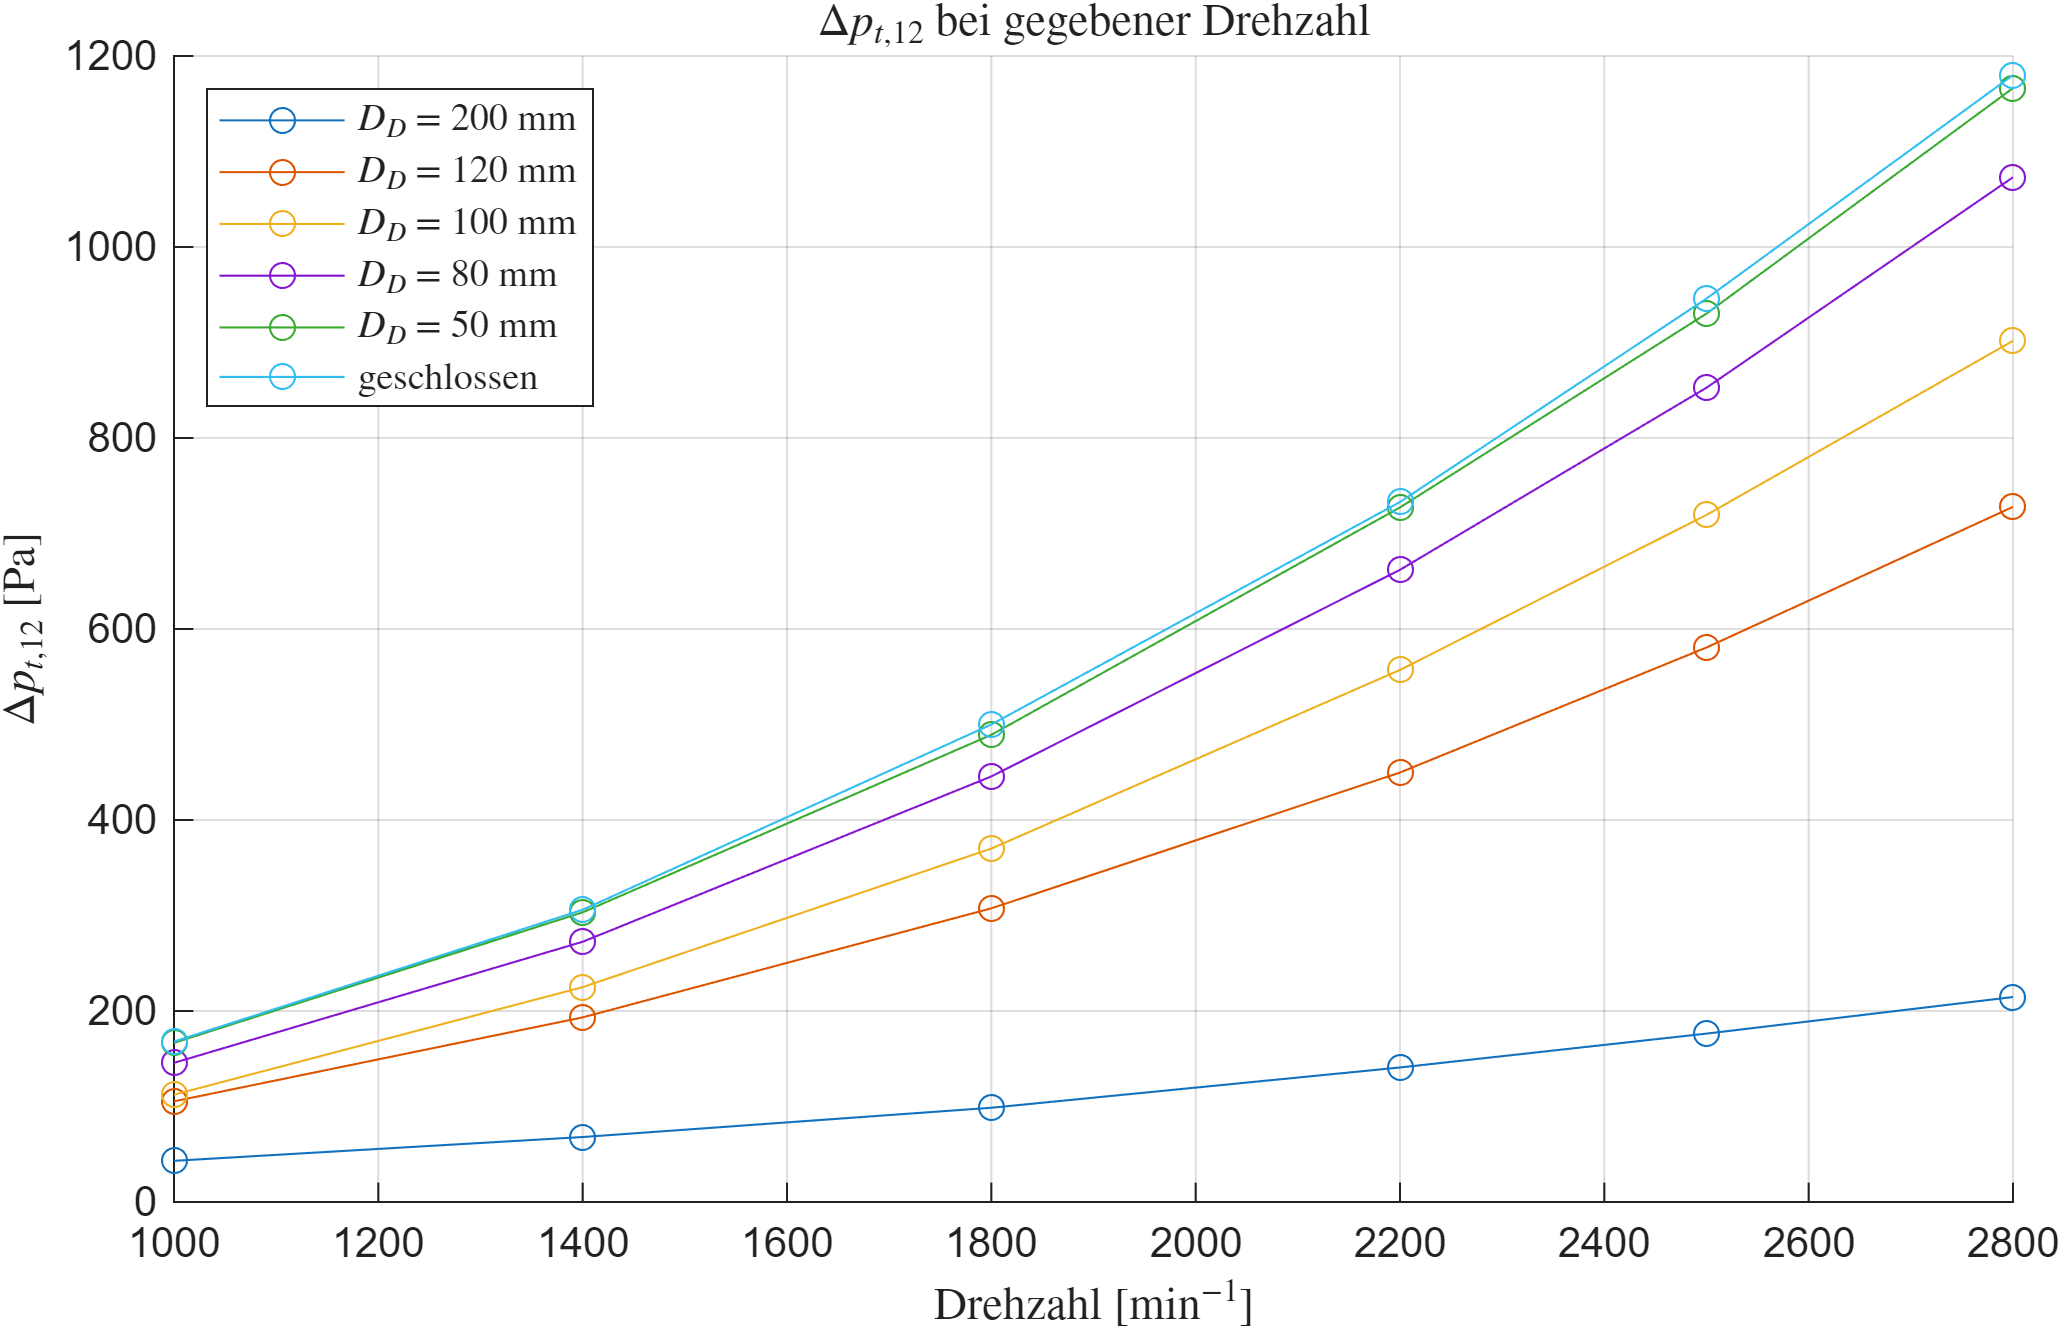
\includegraphics[width = \linewidth]{Plots/Gebläse/Delta_p.png}
    \caption{Totaldruckerhöhung in Abhängigkeit der Drehzahl}
    \label{plot:delta_p_N}
\end{figure}

Berechnung der Wellenleistung:
\begin{equation}
    P_W = M_W \cdot \Omega = M_W \cdot 2\pi \cdot n 
\end{equation}

\begin{equation*}
    P_W = 2,43 \ Nm \cdot 2\pi \cdot \frac{2500}{60}\frac{1}{s} = 636,17 \ W
\end{equation*}

\begin{figure}[H]
    \centering
    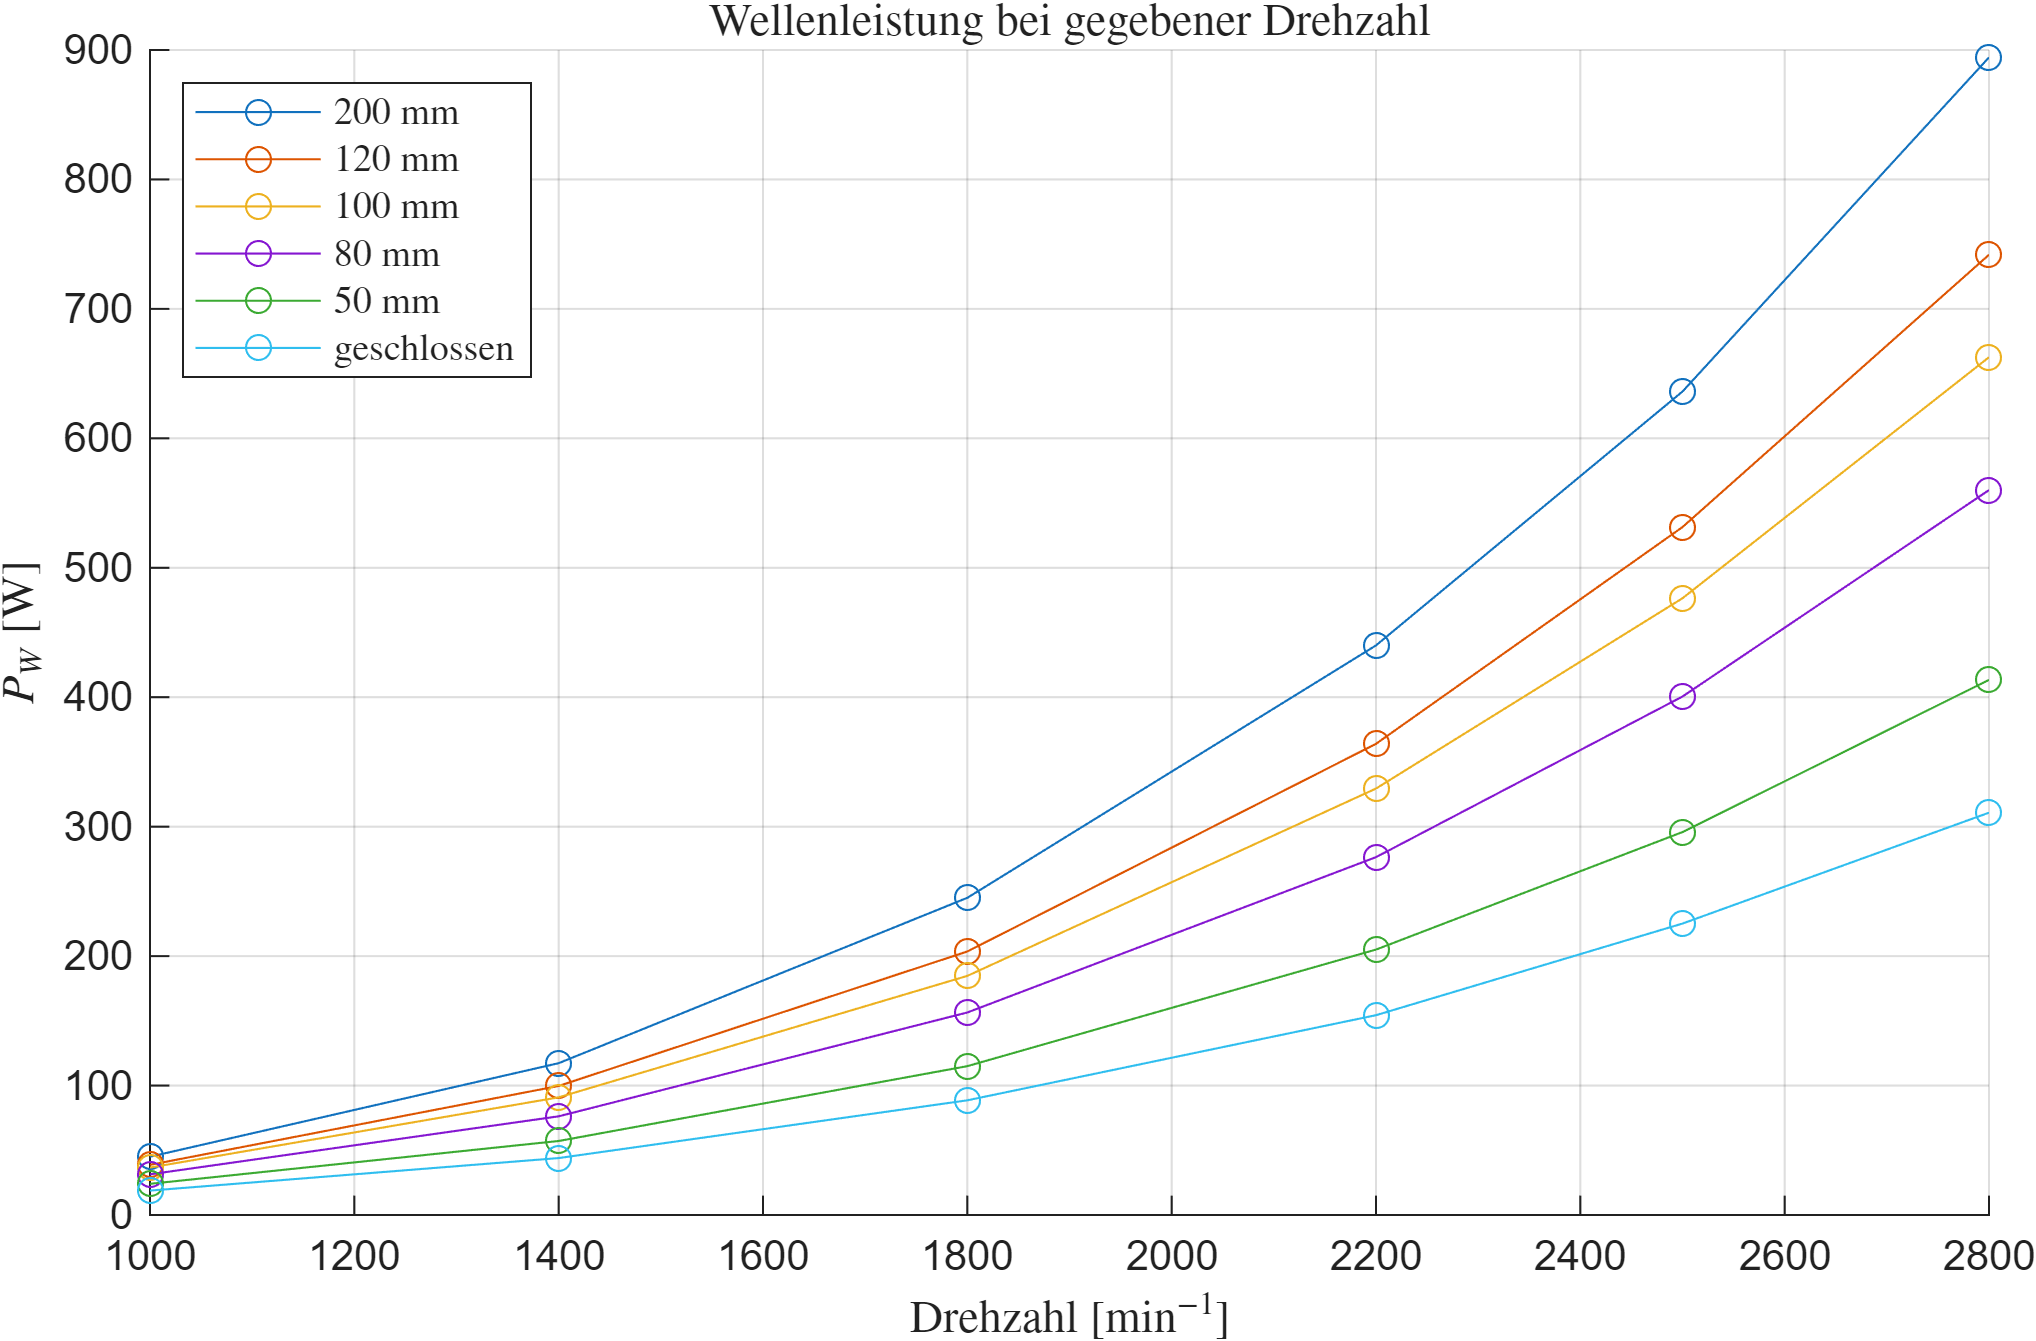
\includegraphics[width = \linewidth]{Plots/Gebläse/P_welle_Plot.png}
    \caption{Wellenleistung in Abhängigkeit der Drehzahl}
    \label{plot:P_welle}
\end{figure}
Mit der Wellenleistung wird der Wirkungsgrad berechnet: 
\begin{equation}
    \eta_{fluid} = \frac{P_{fluid}}{P_{mech}}=\frac{\Delta p_{t,12} \cdot \dot V}{P_W}
\end{equation}
\begin{equation*}
    \eta_{fluid} = \frac{176,31 \ Pa \cdot 0,435 \ \frac{m^3}{s}}{636,17 \ W} = 0,1206 \; \widehat= \ 12,1 \ \%
\end{equation*}
Im folgenden Plot werden die Kennlinien wieder sichtbar. Wichtig hierbei ist, dass diesmal die Drehzahl über die Linien konstant ist und sich die Düsenöffnungen ändern:
\begin{figure}[H]
    \centering
    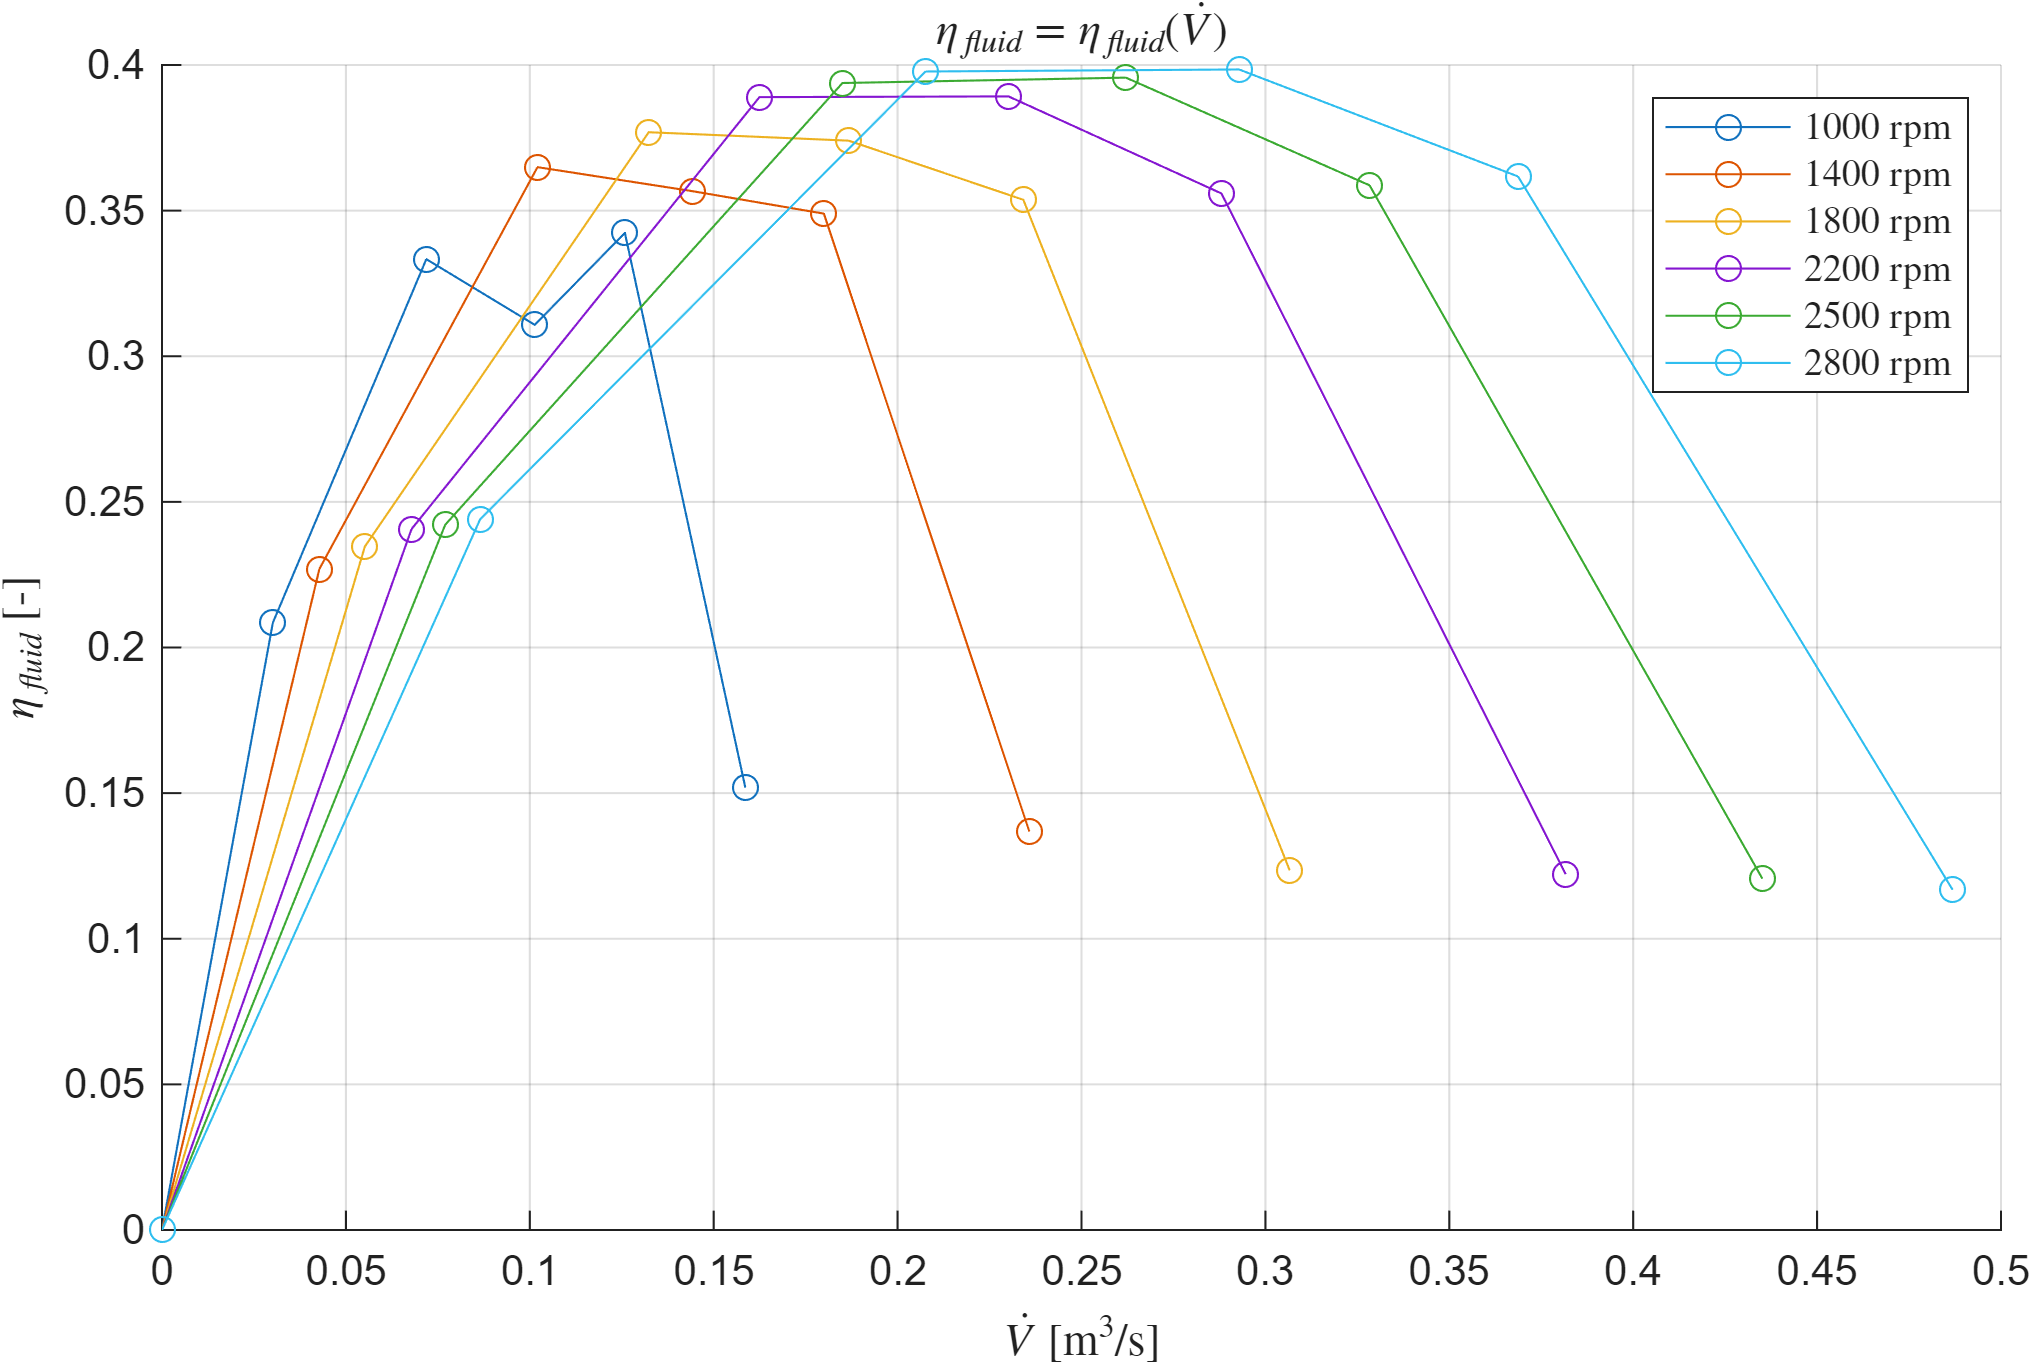
\includegraphics[width = 0.8\linewidth]{Plots/Gebläse/eta_plot.png}
    \caption{Strömungsmechanischer Wirkungsgrad in Abhängigkeit des Volumenstroms}
    \label{plot:eta_plot}
\end{figure}
\noindent
Zusätzlich wird ein Muscheldiagram erstellt, mithilfe von griddata in Matlab. Damit werden Flächen mit konstantem Wirkungsgrad sichtbar:
\begin{figure}[H]
    \centering
    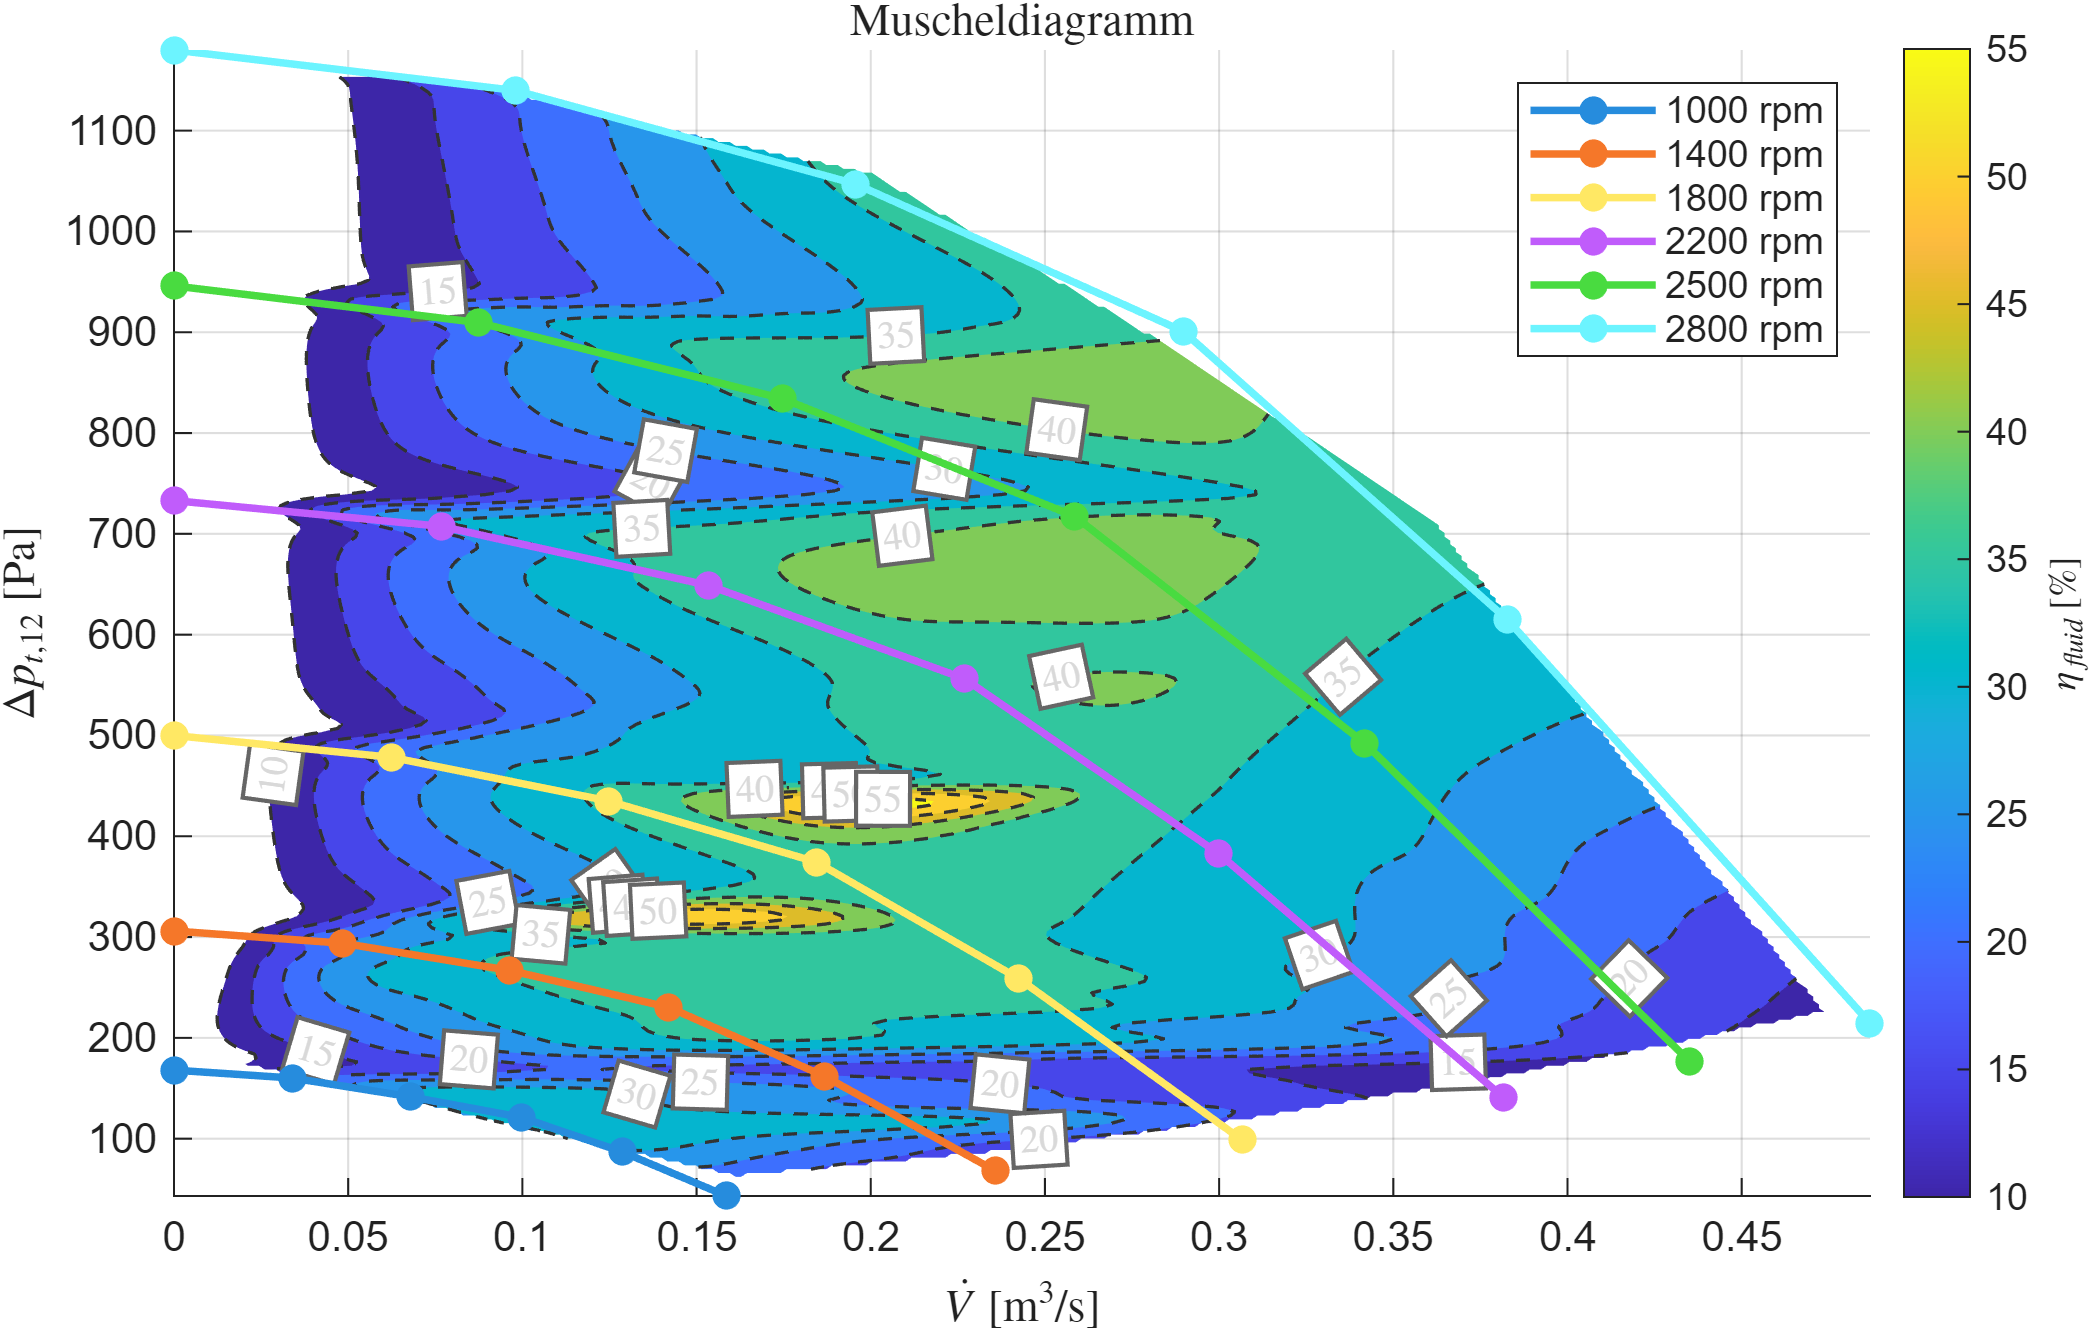
\includegraphics[width=0.8\linewidth]{Plots/Gebläse/Muscheldiagramm.png}
    \caption{Muscheldiagramm des Radialgebläses}
    \label{plot:Muscheldiagram}
\end{figure}
Zuletzt werden die dimensionslosen Kennzahlen, Lieferzahl $\varphi$ und die Druckziffer $\Psi$ ermittelt: 
\begin{equation}
    \varphi = \frac{\dot V}{\frac{\pi^2}{4}\cdot D_L^3 \cdot n}
\end{equation}
\begin{equation*}
    \varphi = \frac{0,435 \ \frac{m^3}{s}}{\frac{\pi^2}{4}\cdot (0,5\ m)^3 \cdot (\frac{2500}{60}\frac{1}{s})} = 0,0338
\end{equation*}

\begin{equation}
    \Psi = \frac{\Delta p_{t,12}}{\frac{\rho}{2}\cdot \pi^2 \cdot D_L^2 \cdot n^2}
\end{equation}
\begin{equation*}
    \Psi = \frac{176,31 \ Pa}{\frac{1,137\ \frac{kg}{m^3}}{2}\cdot \pi ^2 \cdot (0,5 \ m )^2 \cdot (\frac{2500}{60}\frac{1}{s})^2} = 0,0724
\end{equation*}
Plottet man nun diese Kennzahlen sieht man, dass alle übereinander liegen:
\begin{figure}[H]
    \centering
    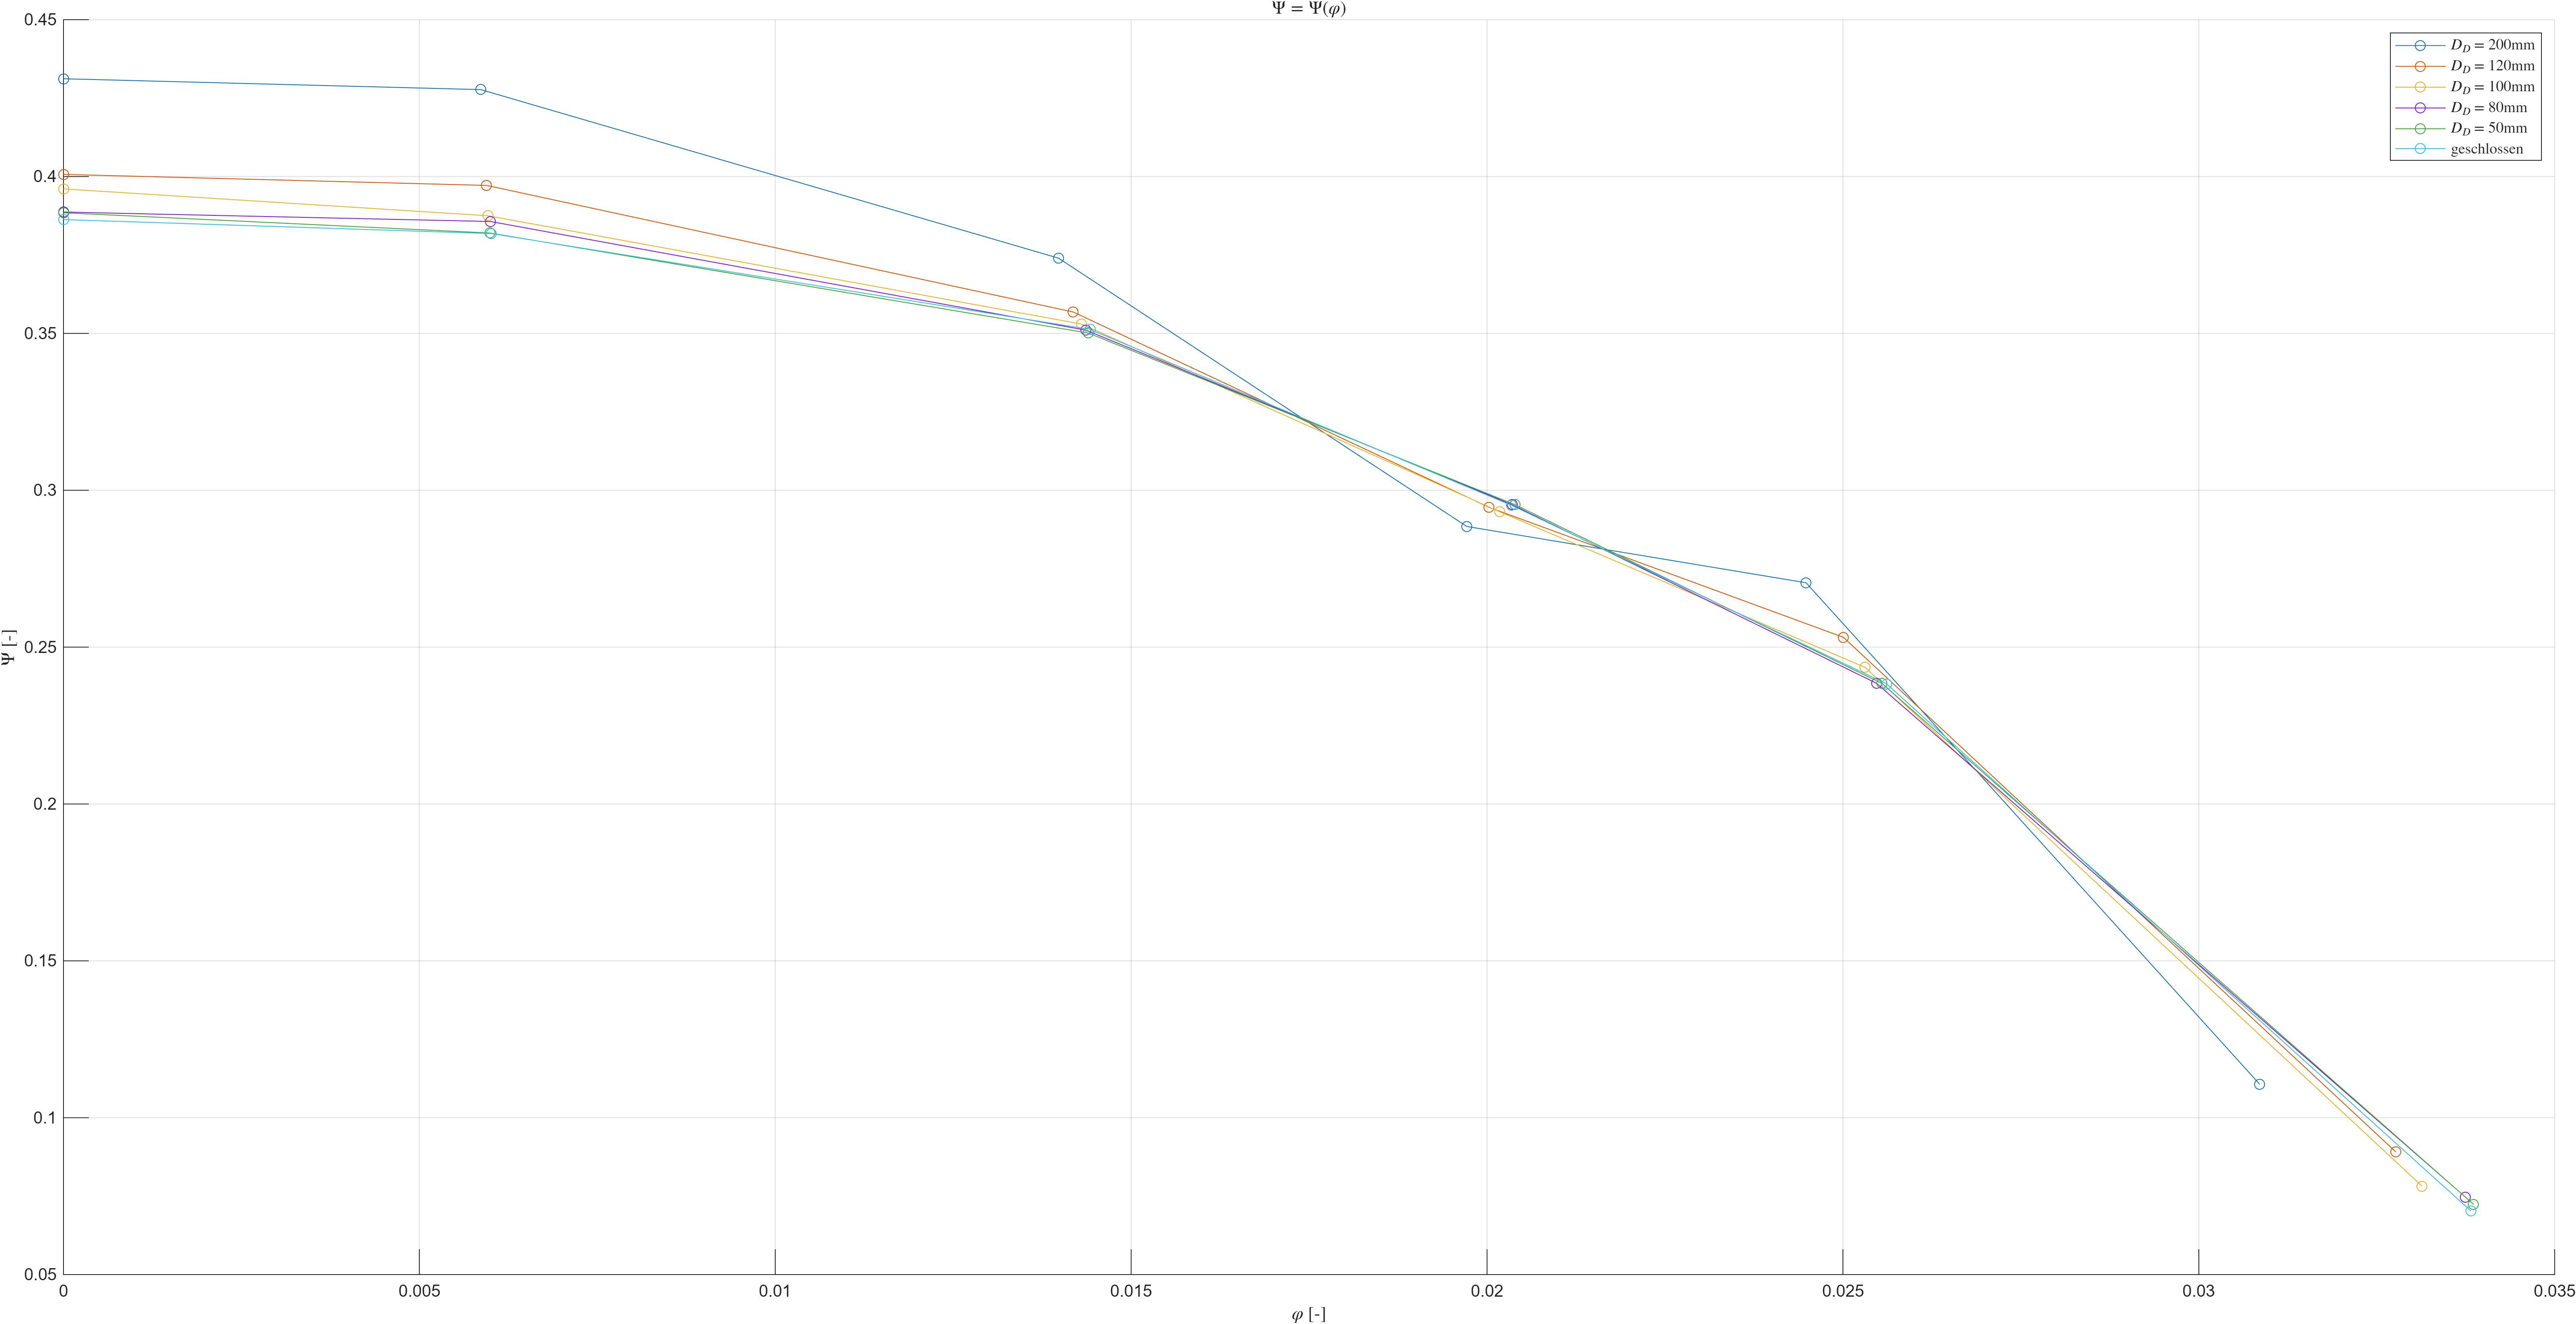
\includegraphics[width=\linewidth]{Plots/Gebläse/Psi_plot.png}
    \caption{Druckziffer in Abhängigkeit der Lieferzahl}
    \label{plot:Psi}
\end{figure}

\subsection{Interpretation der Ergebnisse}
Die experimentell gemessenen Messpunkte zeigen insgesamt ein physikalisch konsistentes Verhalten. Diese 
decken sich gut mit den theoretischen Ähnlichkeitsgesetzen aus dem Lehrbuch \cite{Lehrbuch}. %Hier skript oder Lehrbuch referenzieren
Der Volumenstrom steigt bei allen Drosselkonfigurationen, wie in Plot \ref{plot:Volumenstrom} sichtbar, linear mit der Drehzahl an. Dies entspricht genau den dem Ähnlichkeitsgesetz
$\dot{V} \propto N$. Ebenso ist ersichtlich, dass bei kleineren Düsenöffnungen der Volumenstrom niedriger wird, dies lässt sich durch höheren Strömungswiderstand erklären. \\
Die Totaldruckerhöhung steigt mit der Drehzahl quadratisch an. Dies entspricht ebenso dem
\\ Ähnlichkeitsgesetz $\Delta p \propto N^2$.
In Plot \ref{plot:delta_p_N} ist zu erkennen, dass der Druck mit abnehmenden Düsenöffnungen steigt. Dies ist ein
intuitives Verhalten und kommt den theoretischen Berechnung nahe. \\
Die Wellenleistung in Plot \ref{plot:P_welle} steigt auch wie die theoretische Ähnlichkeitsgesetze an mit $P_{W} \propto N^3$.
Zu sehen ist, dass bei offenen Rohr die Leistung am höchsten ist, da dort der größte Volumenstrom gefördert wird. Während bei geschlossenem Rohr nur
die Reibungs und Ventilationsverluste kompensiert werden müssen.\\
Der strömungsmechanische Wirkungsgrad $\eta$ in Plot \ref{plot:eta_plot} zeigt ein Maximum bei mittleren Drosselungen und höheren
Drehzahlen. Es ist zu sehen dass, das Maximum bei allen Variationen auf ca $40 \%$ begrenzt ist. Bei geschlossenen Rohr
ist der Wirkungsgrad definitionsgemäß Null, da kein Volumenstrom erzeugt wird. Bei offenen Rohr ist der Wirkungsgrad gering,
da die Totaldruckerhöhung in diesem Falle sehr gering ist. Dieses Verhalten und die Kennlinien sind sehr ähnlich zu den theoretisch
behandelten Kennlinien im Lehrbuch \cite{Lehrbuch}.\\
Das Muscheldiagram \ref{plot:Muscheldiagram} zeigt, dass der maximale erreichbare Wirkungsgrad bei $\eta = 55 \%$ liegt. Dementsprechend müssten die Drehzahlen bzw. Drosselungen feiner angepasst werden um diesen optimalen Betriebspunkt zu finden. Ebenso ist zu sehen, dass die
Kennlinien für $\Delta p_{t,12}$ eine sehr gute Muschelform ergeben und auch sehr ähnlich zu Lehrbuch Kennlinien sind. \\
Bei den dimensionslosen Kennzahlen in Plot \ref{plot:Psi} ist zu sehen, dass alle Kennlinien auf nahezu einer Linie zusammen
fallen. Auch das liegt wiederum sehr nah an theoretischen Kennlinien aus dem Lehrbuch \cite{Lehrbuch}. Die geringen Abweichungen lassen sich auf Messwertgenauigkeiten zurückführen. \\
Hinsichtlich der Messwertgenauigkeiten ist anzumerken, dass die Geschwindigkeitsmessung am Düsenaustritt nur punktuell gemessen wird. Das lässt keine 
vollständige Messung des Geschwindigkeitsprofil zu. Der Korrekturfaktor $k_1$ wird verwendet um dies auszugleichen, ist aber dennoch nicht
zu $100 \%$ korrekt. \\
Insgesamt lässt sich aufgrund des sehr ähnlichen Verhalten der experimentellen Werte zu den theoretischen Werten eine stark repräsentative
Kennlinie für das Gebläse erschließen. 
%Leistungsziffer $\lambda$:
%\begin{equation}
%    \lambda = \frac{\phi \cdot \Psi}{\eta_{fluid}} 
%\end{equation}
%
%\begin{equation*}
%    \lambda = \frac{0,0338\cdot 0,0724}{0,1206}= 0,0203
%\end{equation*}
%
%\subsection{Interpretation der Ergebnisse}
\clearpage
\newpage
\section{Venturi}
\subsection{Einleitung / Abstract}
Im folgenden Versuch wird das Druck- und Geschwindigkeitsverhalten einer Strömung innerhalb eines Venturi-Rohrs analysiert. Auf experimentellem und theoretischem Weg werden im Verlauf des Rohrs die Druckwerte, der Druckbeiwert und die Geschwindigkeit ermittelt und anschließend graphisch ausgewertet und verglichen.

\subsection{Versuchsbeschreibung und -durchführung}
Der Venturi-Versuch dient der Charakterisierung der Strömung in einem Venturi-Rohr, welches häufig zur effizienten Messung von Volumen- und Massenströmen eingesetzt wird. Durch einen Diffusor stromab der engsten Stelle wird kinetische Energie (dynamischer Druck) teilweise wieder in statischen Druck zurückgewandelt, was den bleibenden Druckverlust im Vergleich zu Messblenden minimiert.
\subsubsection{Versuchsaufbau}
Die Versuchsanlage besteht aus einem Axialgebläse, das Luft aus der Umgebung ansaugt und in eine Beruhigungskammer fördert. Das anschließende Venturi-Rohr setzt sich aus einer Düse, einem Rohrabschnitt mit engstem Querschnitt und einem Diffusor zusammen. Zur Bestimmung des Durchflusses ist an Position (0) ein auf die Rotationsachse ausgerichtetes Prandtl-Rohr verbaut, welches an ein Schrägrohrmanometer zur Messung des dynamischen Drucks angeschlossen ist. Entlang der Rohrwand befinden sich an den Positionen (1) bis (8) Messstellen zur Abnahme der statischen Drücke. Diese Wanddrücke werden mit einer DMS-Druckmessdose relativ zum Umgebungsdruck gemessen.

\begin{figure}[h]
    \centering
    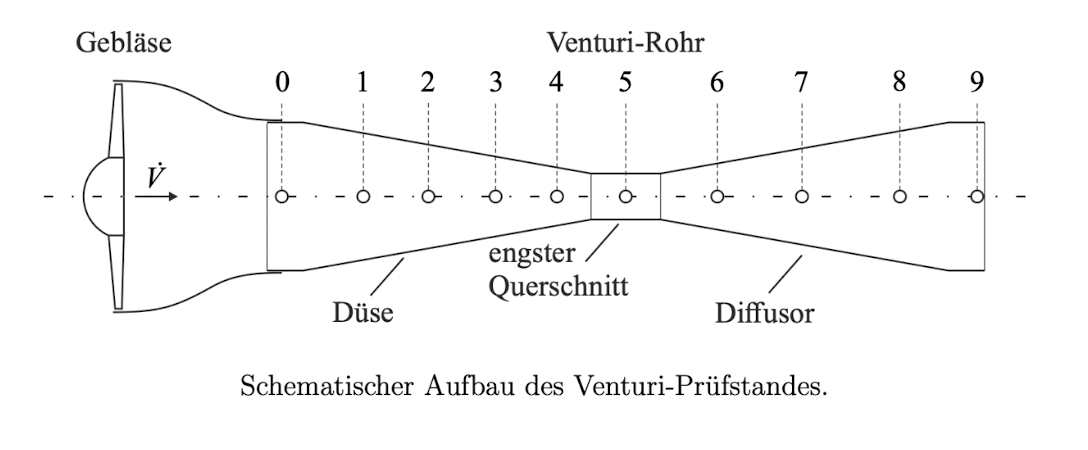
\includegraphics[width=0.9\textwidth]{Bilder/Versuchsaufbau_Venturi.png}
    \caption{Versuchsaufbau Venturi}
    \label{fig:versuchsaufbau_venturi}
\end{figure}

\subsubsection{Versuchsdurchführung}
Während des Versuchs wird das Axialgebläse mit einer konstanten Drehzahl betrieben, um Luft durch das Venturi-Rohr zu fördern. Es wird dabei ein spezifischer Betriebspunkt untersucht, für den zunächst der Messwert des dynamischen Drucks am Schrägrohrmanometer notiert wird. Anschließend werden die statischen Wanddrücke an den verschiedenen Messstellen nacheinander erfasst. Hierzu wird ein Multiplexer (Revolver) verwendet, um die einzelnen Druckanschlüsse nacheinander auf das digitale Druckmessgerät zu schalten. Die Messwerte werden zusammen mit den zugehörigen Positionen und Rohrdurchmessern für die spätere Auswertung dokumentiert.

\subsection{Versuchsergebnisse}
Für die Errechnung der Versuchsergebnisse werden auch hier wieder die aktuellen Tageswerte benötigt.
\begin{table}[h]
\centering
\begin{tabular}{lr}
\hline
\textbf{Parameter} & \textbf{Wert} \\
\hline
Luftdruck $p_L$ & 95550 Pa \\
Umgebungstemperatur $T$ & 292,75 K \\
Relative Luftfeuchtigkeit $\varphi_L$ & 38 \% \\
\hline
\end{tabular}
\caption{Tageswerte der Lufteigenschaften}
\end{table}

Aus dem gemessenen Werten und der spezifischen Gaskonstante $R_S=287,05 \frac{J}{kg \cdot K}$ lässt sich die Luftdichte errechnen.
\begin{equation*}
    \varrho = \frac{95545 \ Pa}{287,05 \ \frac{J}{kgK} \cdot 292,75 \ K}=1.137 \frac{kg}{m^3}
\end{equation*}
Die an den Messpunkten 1-8 gemessenen Differenzdrücke wurden in Tabelle \ref{fig:Venturi-Werte} eingetragen. Der statische Druck $p_0$ wird ermittelt, indem eine lineare Extrapolation aus den Folgedrücken $p_1$ und $p_2$ durchgeführt wird.
\begin{equation*}
    p_0=p_1+\frac{p_2-p_1}{105mm-45mm}\cdot (0mm-45mm)= 300 Pa
\end{equation*}
Für die Berechnung des Volumenstroms $\dot{V}$ wird die lokale Querschnittsfläche $A_i(0)$ und Strömungsgeschwindigkeit $u(0)$ an der Messstelle 0 benötigt. Die Strömungsgeschwindigkeit wird mithilfe der berechneten Luftdichte $\varrho$ und dem dynamischen Druck, welcher mit dem Schrägrohrmanometer gemessen wurde, errechnet.
\begin{equation*}
    A_i(0) = \pi \left( \frac{d_i}{2} \right)^2 = \pi \left( \frac{0.104}{2} \right)^2 = 0.0085m^2
\end{equation*}
\begin{equation*}
    u(0)= \sqrt{\frac{2 \cdot p_{0,dyn}}{\varrho}}= \sqrt{\frac{2 \cdot 40Pa}{1.137 \frac{kg}{m^3}}}=8.39 \frac{m}{s}
\end{equation*}
\begin{equation*}
    \dot{V}=u(0) \cdot A_i(0) = 0.0713 \frac{m^3}{s}
\end{equation*}

Aus dem Volumenstrom $\dot{V}$ und den lokalen Querschnittsflächen entlang der Strecke des Venturi-Rohrs lässt sich mit folgender Formel die theoretische Geschwindigkeit errechnen und in einem Graphen über die Position x darstellen (Abbildung \ref{fig:Venturi_Geschwindigkeit}).

\begin{equation*}
    u_{i,theor}=\frac{\dot{V}}{A_i}
\end{equation*}



In der Abbildung \ref{fig:Venturi_Druckverlauf} sind der gemessene Druck $p(x)$ und der errechnete theoretische Druck $p_{theor}(x)$ dargestellt.
\begin{equation*}
    p_{theor}(x)=p_0 + \frac{\varrho}{2}\cdot(u_0^2-u_{i,theor}^2)
\end{equation*}


Zuletzt wird aus den gemessenen Drücken $p_i$ und $p_{0,dyn}$, dem errechneten Referenzdruck $p_0$ und den theoretischen Drücken $p_{i,theor}$ der Druckbeiwert $c_p$ und der theoretische Druckbeiwert $c_{p,theor}$ über die Strecke $x$ berechnet und in der Abbildung \ref{fig:Venturi_cp} dargestellt.
\begin{equation*}
    c_p=\frac{p_i-p_0}{p_{0,dyn}}
\end{equation*}
\begin{equation*}
    c_{p,theor}=\frac{p_{i,theor}-p_0}{p_{0,dyn}}
\end{equation*}

\begin{figure}[h]
    \centering
    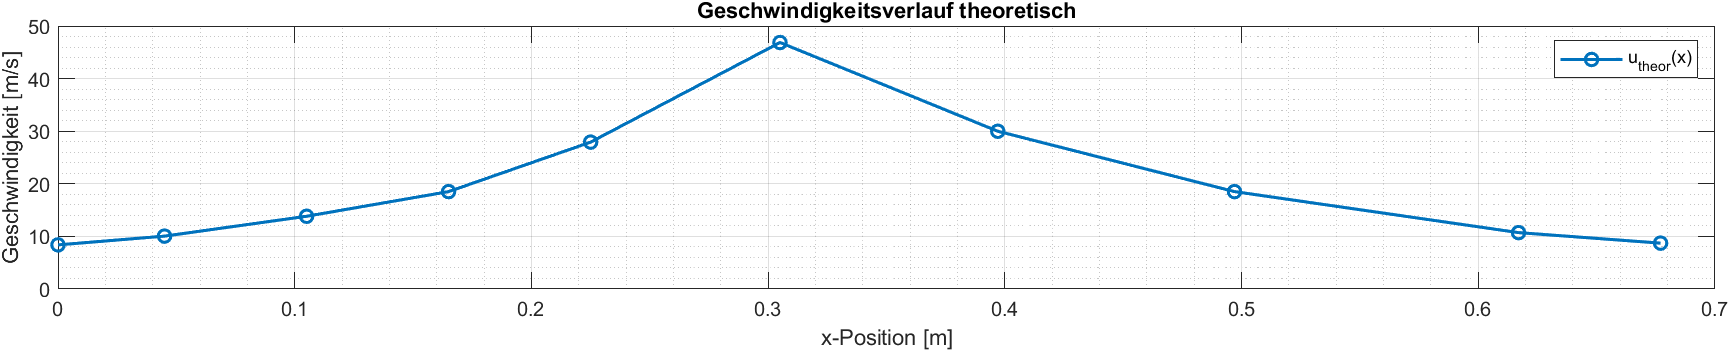
\includegraphics[width=\textwidth]{Plots/Venturi/Geschwindigkeit.png}
    \caption{Theoretischer Geschwindigkeitsverlauf}
    \label{fig:Venturi_Geschwindigkeit}
\end{figure}

\begin{figure}[h]
    \centering
    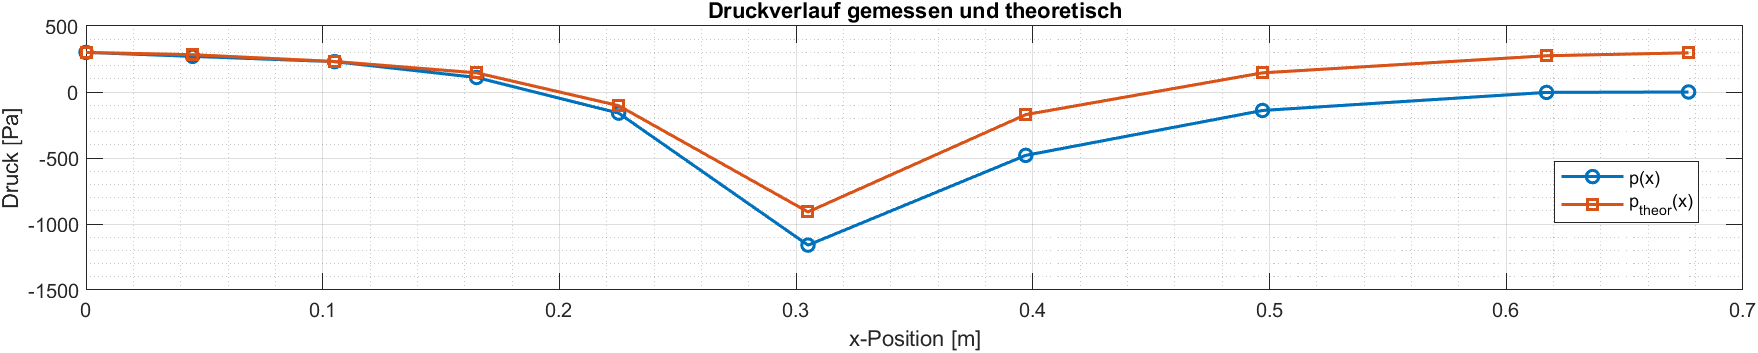
\includegraphics[width=\textwidth]{Plots/Venturi/Druckverlauf.png}
    \caption{Experimenteller und theoretischer Druckverlauf}
    \label{fig:Venturi_Druckverlauf}
\end{figure}

\begin{figure}[h]
    \centering
    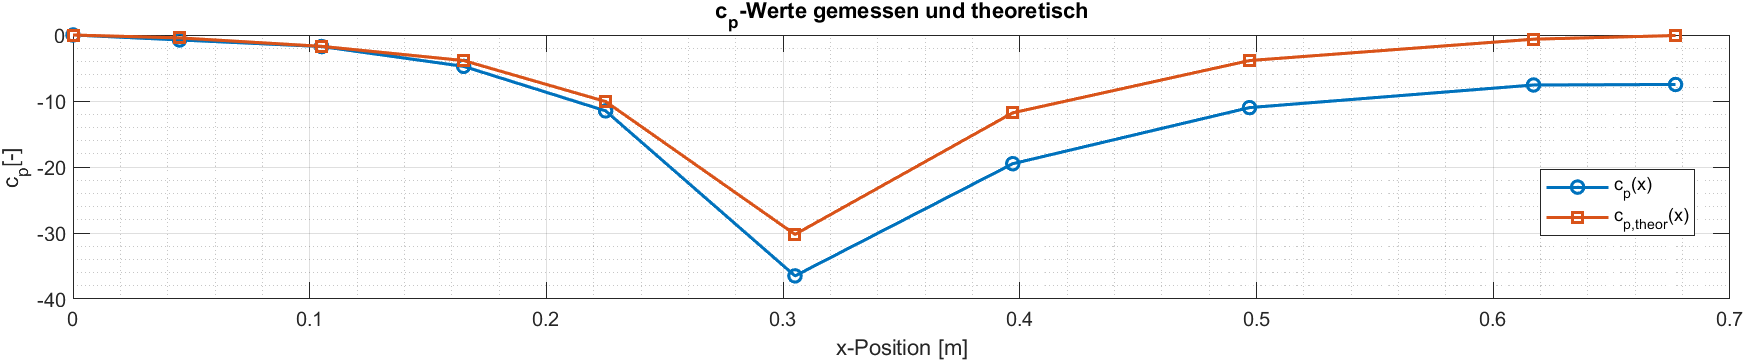
\includegraphics[width=\textwidth]{Plots/Venturi/cp.png}
    \caption{Experimenteller und theoretischer Verlauf des Druckbeiwerts}
    \label{fig:Venturi_cp}
\end{figure}
\subsection{Interpretation der Ergebnisse}
Die Auswertung der Druck- und Geschwindigkeitsverläufe entlang des Venturi-Rohrs zeigt die erwartete Druckabsenkung in der Rohr-Engstelle zusammen mit einer Beschleunigung der Strömung. Im Bereich des Diffusors sinkt die Geschwindigkeit der Strömung wieder und der statische Druck nimmt wieder zu. Die berechneten, theoretischen Werte basieren auf der Annahme einer reibungsfreien, inkompressiblen Strömung mit gleichmäßigem Geschwindigkeitsprofil. Die jeweiligen Graphen der theoretischen und experimentell gemessenen Werte zeigen einen sehr ähnlichen Verlauf. Die Abweichung der beiden Verläufe zeigt den Einfluss der real auftretenden Effekte von Reibungsverlusten und Strömungsablösungen im Diffusor. Durch diese Einflüsse liegen die realen Druckwerte innerhalb des Venturirohrs unterhalb der theoretischen Werte und der auch der Endwert des Drucks liegt unterhalb des Startwerts.

%\subsection{Anhang Venturi Berechnungen}
%\subsubsection{Messung}
%\begin{figure}[H]
%    \centering
%    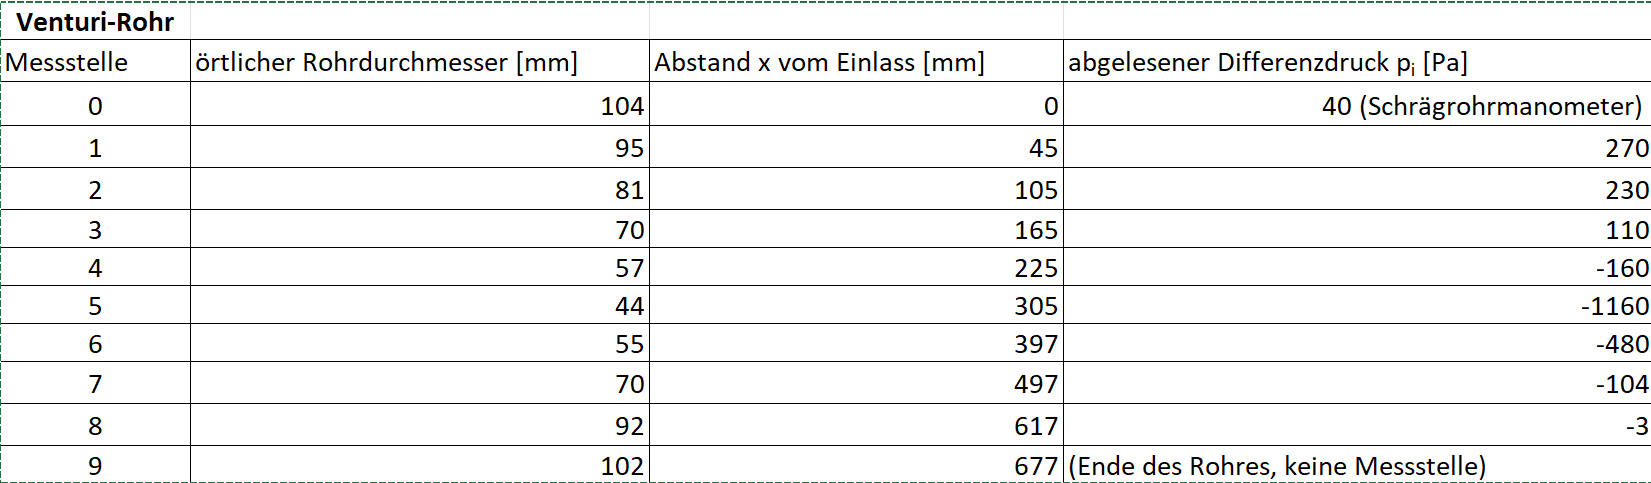
\includegraphics[width=\textwidth]{Bilder/Venturi_Werte.png}
%    \caption{Wertetabelle Venturi}
%    \label{fig:Venturi-Werte}
%\end{figure}
\section{Anhang}
\subsubsection*{Messwerte}
\begin{figure}[H]
    \centering
    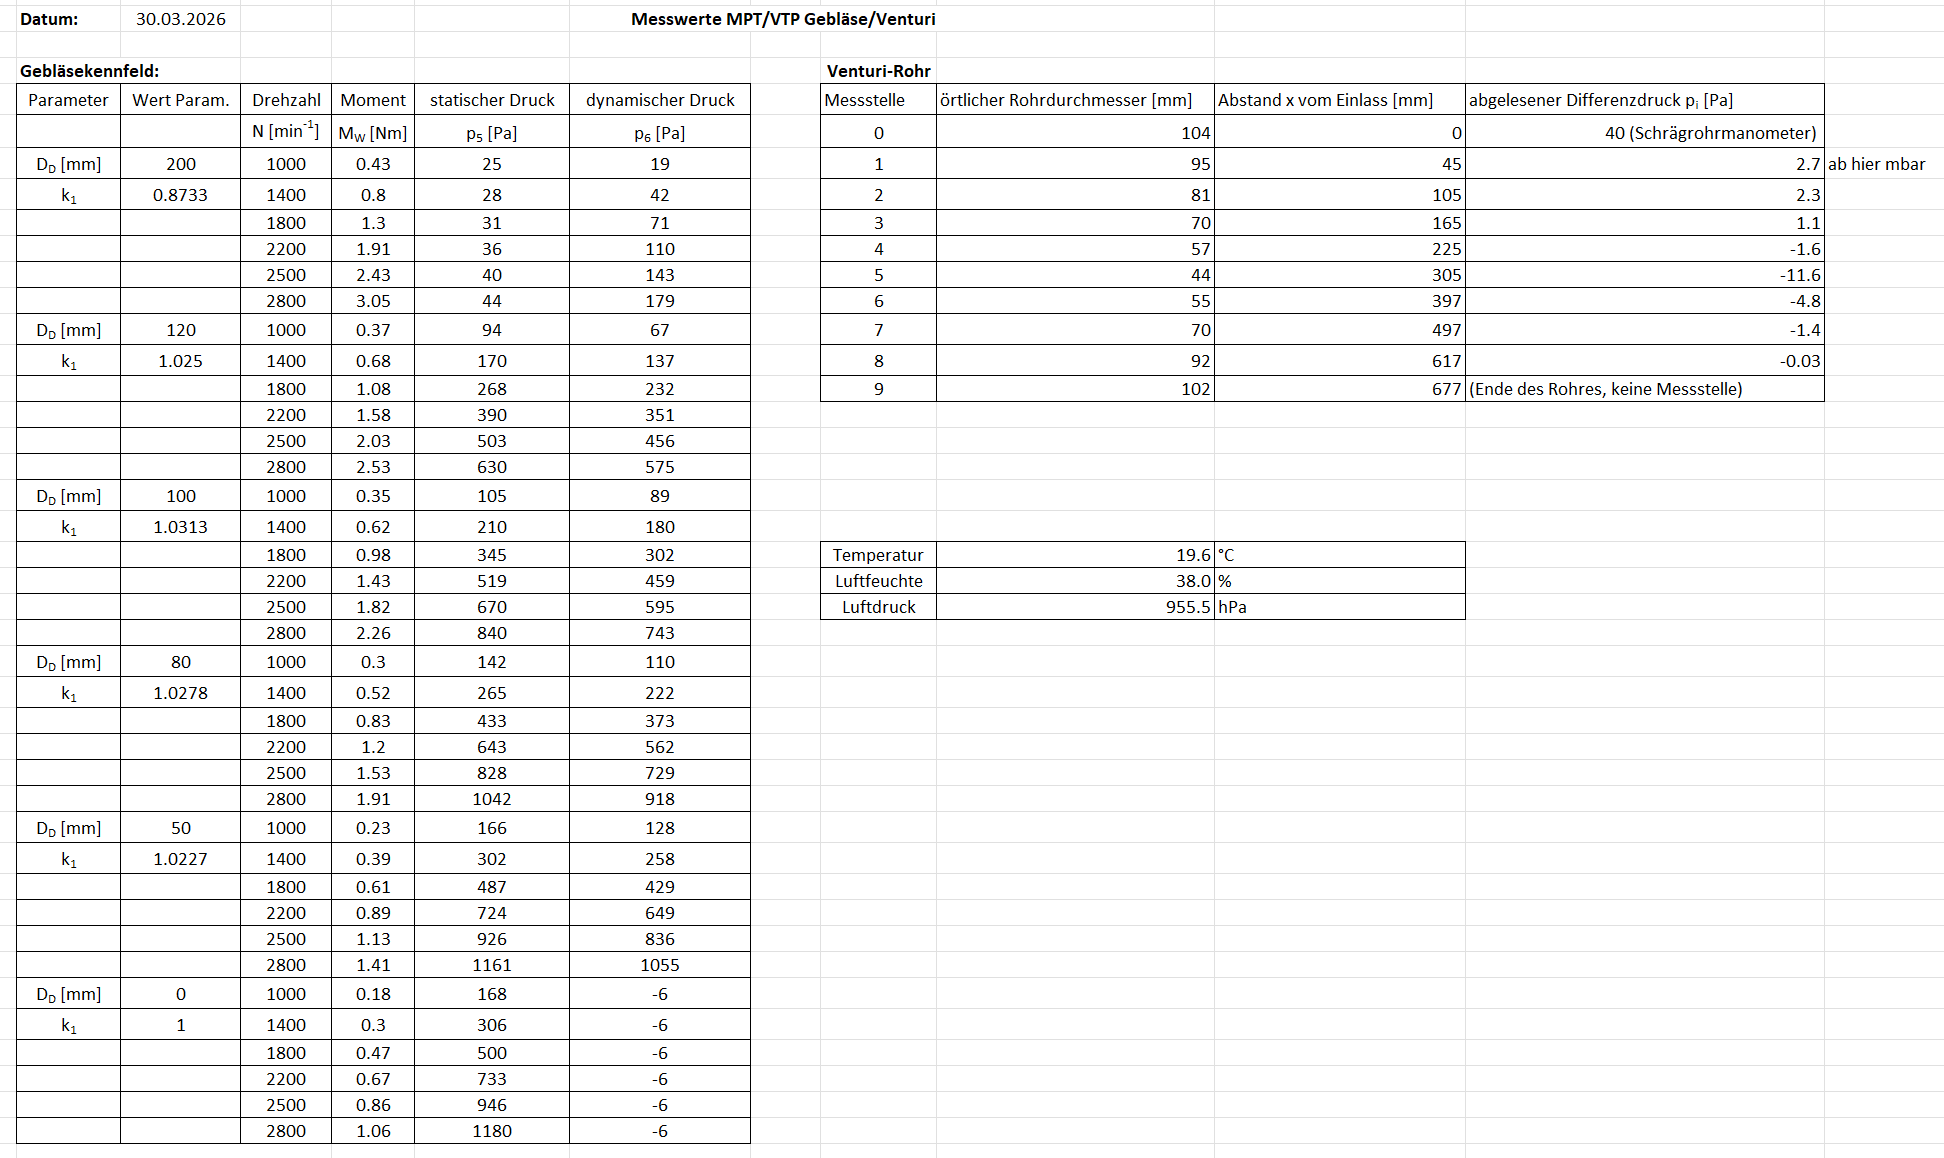
\includegraphics[scale=0.35, angle=90]{Bilder/Messwerte.png}
    \caption{Messwerte Gebläse und Venturi}
    \label{fig:Messwerte}
\end{figure}
\newpage
\subsubsection*{MATLAB-Code Gebläse}
\begin{lstlisting}[language=Matlab, caption={Berechnung und Plot des Volumenstroms $\dot{V}$}, label={code:V_dot}]
    %% Berechnung_V_dot.m
N=[1000 1400 1800 2200 2500 2800]';

D_D=[0.200 0.120 0.100 0.080 0.050 0];

%% Staudruck nach Diffusor
p_6=[19	42 71 110 143 179 67 137 232 351 456 575 89 180 302	459	595	743	110	222	373	562	729	918	128	258	429	649	836	1055 0 0 0 0 0 0];
p_6_mat=reshape(p_6,6,6);
% Zeilen = Duesen, Spalten = Drehzahlen

%% Statischer Druck vor Diffusor
p_5=[25	28 31 36 40 44 94 170 268 390 503 630 105 210 345 519 670 840 142 265 433 643 828 1042 166 302 487 724 926 1161	168	306	500	733	946	1180];
p_5_mat=reshape(p_5,6,6);

%% Drehmoment an Welle
M_welle=[0.43 0.8 1.3 1.91 2.43 3.05 0.37 0.68 1.08 1.58 2.03 2.53 0.35 0.62 0.98 1.43 1.82 2.26 0.3 0.52 0.83 1.2 1.53 1.91 0.23 0.39 0.61 0.89 1.13 1.41 0.18 0.3 0.47 0.67 0.86 1.06];
M_welle_mat=reshape(M_welle,6,6);

k_1=[0.8733 1.025 1.0313 1.0278 1.0227 1];

p_inf = 95545;
T     = 292.75;
R_S   = 287.05;
rho   = p_inf/(R_S*T);

%% Geschwindigkeit & Volumenstrom
c_6_mat = sqrt(2/rho .* p_6);

i=1;
d=1;
while i <=36
    A_D(d)=pi*D_D(d)^2/4;
    V_dot(i) = k_1(d) .* c_6_mat(i) .* A_D(d);
    if mod(i,6)==0
        d=d+1;
    end
    i=i+1;
end
V_dot_mat = reshape(V_dot, 6, 6);

%% Plot V_dot ueber N
figure
hold on
for d = 1:6
    plot(N, V_dot_mat(:,d), 'o-');
end
...
\end{lstlisting}
\begin{lstlisting}[language=Matlab, caption={Berechnung und Plot der Totaldruckerhöhung $\Delta p_{t,12}$}, label={code:delta_p}]
    %% Berechnung_delta_pt_12.m
Berechnung_V_dot

%% Berechnung
c_5_mat = V_dot_mat ./ (pi * 0.2^2 / 4);
pt_12_mat = 1.25 * rho/2 .* c_5_mat.^2 + p_5_mat;

%% Plot pt_12 ueber Drehzahl
figure
hold on
for d = 1:6
    
    plot(N, pt_12_mat(:,d), 'o-');
end
...
\end{lstlisting}
\begin{lstlisting}[language=Matlab, caption={Berechnung und Plot der Wellenleistung $P_W$, des Wirkungsgrades und des Muscheldiagramms}, label={code:P_W} ]
%% Berechnung_P_welle.m
Berechnung_delta_pt_12

%% Wellenleistung
omega = (2*pi/60) * [1000 1400 1800 2200 2500 2800]';% (6x1)
for i=1:6
    P_welle_mat(:,i) = M_welle_mat(:,i) .* omega;
end

%% Plot 1: P_welle ueber Drehzahl
figure
hold on
for d = 1:6
    plot(N, P_welle_mat(:,d), 'o-');
end
...

%% Wirkungsgrad
 eta_mat = (pt_12_mat .* V_dot_mat) ./ P_welle_mat;

%% Plot 2: eta ueber V_dot
figure
hold on
for n = 1:6
    v = V_dot_mat(n,:);
    e = eta_mat(n,:);
    plot(v, e, 'o-');
end
...

%% Muscheldiagramm
x = V_dot_mat(:);
y = pt_12_mat(:);
z = eta_mat(:);
 
x_grid = linspace(min(x), max(x), 300);
y_grid = linspace(min(y), max(y), 300);
[X, Y] = meshgrid(x_grid, y_grid);
 
% Spline 
Z = griddata(x, y, z, X, Y, 'cubic');
 
% Gauss-Glaettung der Gridflaeche
Z = imgaussfilt(Z, 2);
 
figure
hold on
 
...
 
% Isolinien
[C, h] = contour(X, Y, Z*100, 10:5:80, ...

 ...

% Kennlinien mit Drehzahl
colors = lines(6);
for n = 1:6
    v = (V_dot_mat(n,:));
    p = (pt_12_mat(n,:));
 
    % Glaetten der Kennlinie
    v_s = smooth(v, 3);
    p_s = smooth(p, 3);
 
    plot(v_s, p_s, 'o-',
    ...
end
\end{lstlisting}
\begin{lstlisting}[language=Matlab, caption={Berechnung und Plot der Druckziffer $\Psi$ über die Lieferzahl $\varphi$}, label={code:Psi}]
    %%Daten holen
Berechnung_P_welle

%% Druckziffer Psi
n_rps = N / 60;  % Drehzahl von rpm in 1/s
D_L = 0.5;       % Laufraddurchmesser [m]

% Psi und phi berechnen
for i=1:6
psi_mat(:,i) = pt_12_mat(:,i) ./ (rho/2 * pi^2 * D_L^2 .* n_rps.^2);
phi_mat (:,i)= V_dot_mat(:,i) ./ (pi^2/4 * D_L^3 .* n_rps);
end

%% Plot: Psi ueber phi
figure
hold on
for n = 1:6
    plot(phi_mat(n,:), psi_mat(n,:), 'o-');
end
\end{lstlisting}
\newpage
\subsubsection*{MATLAB-Code Venturi}
\begin{lstlisting}[language=Matlab, caption={Berechnung und Plot des Druckbeiwerts $c_p$, Druckverlauf $p$ und Geschwindigkeitsverlauf $u$}, label={code:cp}]
clc;
clear;
close;

%% Tagesbedingungen
p_L = 955.5 *100;    %Luftfruck in Pa
t_L = 19.6 + 273.15; % Temperatur in Kelvin
R_S = 287.05;        % spez. Gaskonstante

%% Berechnung Luftdichte
rho = p_L/(R_S*t_L);

%% Geometrie
x_i= [0, 0.045, 0.105, 0.165, 0.225, 0.305, 0.397, 0.497, 0.617, 0.677]; % [m]
d_i= [0.104, 0.095, 0.081, 0.070, 0.057, 0.044, 0.055, 0.070, 0.092, 0.102]; % [m]

%% Druckmessung
p_i= [270, 230, 110, -160, -1160, -480, -140, -3, 0]; %[Pa]

%% Extrapolation P_0
p_0 = p_i(1)+((p_i(2)-p_i(1))/(105-45))*(0-45);

%% Einfuegen p_0
p_i = [p_0, p_i];

%% Abgelesener p_0_dyn (Schraegrohrmanometer)
p_0_dyn= 40 ; %[Pa]

%% Berechnung Querschnitt, Geschwindigkeiten, Volumenstrom
A_i=pi.*(d_i/2).^2; % Querschnittsflaeche
u_0 = sqrt(2*p_0_dyn/rho); %Geschwindigkeit in Punkt 0
V_dot = u_0 * A_i(1); % Volumenstrom (konst)

%% Theoretische Geschwindigkeit
u_i_theo = V_dot ./A_i; % Theoretische Geschwindigkeit

%% theoretische Druecke
p_i_theo = p_0 + rho/2*(u_0^2-u_i_theo .^2); %theoretischer Druckverlauf

%% cp-Werte
cp=(p_i - p_0)/p_0_dyn; % cp Experiment
cp_theo= (p_i_theo - p_0)/p_0_dyn; % cp theoretisch

%% Plots 
figure

% Druecke
subplot (3,1,1)
plot (x_i, p_i, 'o-', 'LineWidth', 1.5)
hold on
plot (x_i, p_i_theo, 's-', 'LineWidth', 1.5)
grid on
grid minor
xlabel('x-Position [m]')
ylabel('Druck [Pa]')
title('Druckverlauf gemessen und theoretisch')
legend('p(x)', 'p_{theor}(x)')
hold off

% cp
subplot (3,1,2)
plot (x_i, cp, 'o-', 'LineWidth', 1.5)
hold on
plot (x_i, cp_theo, 's-', 'LineWidth', 1.5)
grid on
grid minor
xlabel('x-Position [m]')
ylabel('c_{p}[-]')
title('c_{p}-Werte gemessen und theoretisch')
legend('c_{p}(x)', 'c_{p,theor}(x)')
hold off

% Geschwindigkeit
subplot (3,1,3)
plot (x_i, u_i_theo, 'o-', 'LineWidth', 1.5)
grid on
grid minor
xlabel('x-Position [m]')
ylabel('Geschwindigkeit [{m/s}]')
title('Geschwindigkeitsverlauf theoretisch')
legend('u_{theor}(x)')
\end{lstlisting}

\newpage
\newpage
\printbibliography

\end{document}
